\documentclass[a4paper, twoside,openright]{report}

\usepackage[a4paper,top=3cm,bottom=3cm,left=3cm,right=3cm]{geometry} 
\usepackage[fontsize=13pt]{scrextend}
\usepackage[english]{babel}
\usepackage[fixlanguage]{babelbib}
\usepackage[utf8]{inputenc} 
\usepackage[T1]{fontenc}
\usepackage{lipsum}
\usepackage{rotating}
\usepackage{fancyhdr}               

%TODO sembra molto meglio cosi
%\usepackage{lmodern}

\usepackage{amssymb}
\usepackage{amsmath}
\usepackage{amsthm}         

\usepackage{graphicx}
\usepackage[dvipsnames]{xcolor}         
\usepackage{listings}          
\usepackage{hyperref}     
\usepackage[normalem]{ulem}

\pagestyle{fancy}
\fancyhf{}
\lhead{\rightmark}
\rhead{\textbf{\thepage}}
\fancyfoot{}
\setlength{\headheight}{12.5pt}

\fancypagestyle{plain}{
  \fancyfoot{}
  \fancyhead{}
  \renewcommand{\headrulewidth}{0pt}
}

\setlength\parindent{0pt}
\setlength{\parskip}{0.2cm}

\lstdefinestyle{codeStyle}{
    % Colore dei commenti
    commentstyle=\color{teal},
    % Colore delle keyword
    keywordstyle=\color{Magenta},
    % Stile dei numeri di riga
    numberstyle=\tiny\color{gray},
    % Colore delle stringhe
    stringstyle=\color{violet},
    % Dimensione e stile del testo
    basicstyle=\ttfamily\footnotesize,
    % newline solo ai whitespaces
    breakatwhitespace=false,     
    % newline si/no
    breaklines=true,                 
    % Posizione della caption, top/bottom 
    captionpos=b,                    
    % Mantiene gli spazi nel codice, utile per l'indentazione
    keepspaces=true,                 
    % Dove visualizzare i numeri di linea
    numbers=left,                    
    % Distanza tra i numeri di linea
    numbersep=5pt,                  
    % Mostra gli spazi bianchi o meno
    showspaces=false,                
    % Mostra gli spazi bianchi nelle stringhe
    showstringspaces=false,
    % Mostra i tab
    showtabs=false,
    % Dimensione dei tab
    tabsize=2
} \lstset{style=codeStyle}

\lstset{aboveskip=20pt,belowskip=20pt}

\hypersetup{
    colorlinks,
    linkcolor=CornflowerBlue,
    citecolor=CornflowerBlue
}

\newtheorem{definition}{Definizione}[section]
\newtheorem{theorem}{Teorema}[section]
\providecommand*\definitionautorefname{Definizione}
\providecommand*\theoremautorefname{Teorema}
\providecommand*{\listingautorefname}{Listing}
\providecommand*\lstnumberautorefname{Linea}

% --- CONFIGURAZIONE PERFETTA (Multipagina + Testo Piccolo + Flat) ---
\usepackage[most]{tcolorbox}
\tcbuselibrary{listings, skins, breakable} % <--- AGGIUNTO 'breakable'

% Definizione colori
\definecolor{codegray}{rgb}{0.95,0.95,0.95}
\definecolor{codeframe}{rgb}{0.3,0.3,0.3}
\definecolor{keywords}{rgb}{0.6,0,0.4}
\definecolor{comments}{rgb}{0.25,0.5,0.35}
\definecolor{strings}{rgb}{0.5,0,0.5}

\raggedbottom

% -----------------------------------------------------------------
\begin{document}

\begin{titlepage}
\begin{figure}[!htb]
    \centering
    
\includegraphics[keepaspectratio=true,scale=0.5]{images/Frontespizio/cherubinFrontespizio.eps}
\end{figure}

\begin{center}
    \LARGE{UNIVERSITY OF PISA}
    \vspace{5mm}
    \\ \large{DEPARTMENT OF COMPUTER SCIENCE}
    \vspace{5mm}
    \\ \LARGE{Master's Degree in Computer Science}
\end{center}

\vspace{15mm}
\begin{center}
    {\LARGE{\bf AMM Scheduler: \\ \vspace{5mm} \Large Design and Implementation of a \\ Runtime Scheduling System for \\ \vspace{2mm} Asymmetric Heterogeneous Computing}}
\end{center}
\vspace{30mm}

\begin{minipage}[t]{0.47\textwidth}
    {\large{Supervisor:}{\normalsize\vspace{3mm}
    \bf\\ \large{Prof. Marco Danelutto}}}
\end{minipage}
\hfill
\begin{minipage}[t]{0.47\textwidth}\raggedleft
    {\large{Candidate:}{\normalsize\vspace{3mm} \bf\\ \large{Simone Stanganini}}}
\end{minipage}

\vspace{30mm}
\hrulefill
\\\centering{\large{ACADEMIC YEAR 2024/2025}}

\end{titlepage}

\include{chapters/Abstract}

\tableofcontents

%\listoffigures

%\include{chapters/Capitolo1}
\chapter{Introduction}

\section{Contest}
Until a few years ago, performance improvements depended mainly on increasing CPU clock speeds. Today, the approach has changed completely, shifting towards hardware specialization.

Modern computers, from servers to embedded SoCs, don't rely on a single processor anymore. Instead, they integrate different specific accelerators:

\begin{itemize}
    \item \textbf{CPU}: Optimized for sequential tasks and low latency.
    \item \textbf{GPU}: Available as integrated (iGPU) or discrete (dGPU), in a lot of cases both at the same time, designed for massive parallel computing.
    \item \textbf{NPU} (Neural Processing Unit): A recently introduced unit, specialized in speeding up matrix operations for AI.
\end{itemize}

This variety of hardware has created a gap with the software. While hardware offers different resources for different workloads, traditional software tends to be static. It usually assigns tasks to a single device (often just the CPU or GPU) and ignores the other available resources. 

The result is an inefficient use of the system. We could get more throughput with the same efficiency, or be more efficient at the same speed, so the current challenge is \textit{ orchestration}: we need a system that can dynamically map each task to the right accelerator, using the entire heterogeneous topology of the system.

\clearpage 

\section{Objectives}
The main goal of this thesis was to design and implement a scheduler capable of dynamically assigning computational tasks, specifically streams of matrix multiplications, to the different accelerators found in modern architectures.

The work started with an essential preliminary phase. I focused on integrating and studying different compute backends, such as CUDA, SYCL, OpenVINO. This step was useful to create a uniform abstraction layer over the hardware and to verify the technical feasibility of the system.

After this initial phase, the work moved on to the actual development of the scheduler. The core of the project focused on the asymmetric orchestration logic, designed to decide in real-time which resource to use for each specific workload.

Finally, the system was validated with experimental results on a complex hybrid architecture. This setup included an Intel multicore CPU (with integrated GPU and NPU) and a discrete NVIDIA GPU. The tests used to verify the operation were streams of identical matrices, streams of heterogeneous matrices, and splitting larger tasks across multiple accelerators.

\section{Thesis Structure}
The work is organized into the following chapters:

\begin{itemize}
    \item \textbf{Chapter 2}: Introduces the hardware technologies (CPU, GPU, NPU) and the software backends used (CUDA, SYCL, OpenVINO, OpenBLAS).

    \item \textbf{Chapter 3}: Describes the logical design, divided into two phases: the creation of the benchmarking environment and the subsequent design of the scheduler.    

    \item \textbf{Chapter 4}: Details the code implementation. It covers the wrappers for hardware abstraction, the essential data structures for the scheduler (ringbuffer and performance map), and the techniques used for task splitting.

    \item \textbf{Chapter 5}: Analyzes the experimental results, validating the effectiveness of the scheduler on different workloads.

    \item \textbf{Chapter 6}: Draws conclusions on the work done and suggests possible future developments.
\end{itemize}

% CUDA 
% SYCL 
% OEPNVINO 
% OPENBLASS 
% C++/ C Cmake

\chapter{Tools and Technologies}
This chapter presents the hardware and software resources used to develop and validate the system. I chose to work on a hybrid and highly heterogeneous architecture to test the scheduler in a real-world scenario. In this scenario, devices with different performance characteristics and programming models must work together.

\section{Experimental Platform}
All development and benchmarking activities were carried out on a mobile workstation (Lenovo Yoga Pro 9). This platform represents a modern high-performance "Edge" computing node well, it integrates all the types of accelerators studied into a single physical system: multicore CPU, NPU, integrated GPU, and discrete GPU.Having these components available at the same time allowed me to emulate, within a single node, the typical orchestration issues of heterogeneous distributed systems.

\subsection{The SoC: Intel Core Ultra 9 185H}
The core of the system is the Intel Core Ultra 9 185H processor, based on the "Meteor Lake" architecture. This component marks a significant change from traditional monolithic CPUs. It uses a disaggregated design (tiled architecture) that combines different specialized processing units:

\begin{itemize}
    \item \textbf{Host CPU}: This cpu is made of 16 hybrid cores (6 Performance-cores for raw power, 8 Efficient-cores, and 2 Low-Power-cores for background efficiency). In this project, this unit acts as the Host. It runs the scheduler code, manages task dispatching, and coordinates data flows to the accelerators.

    \item \textbf{NPU} - Intel AI Boost: The Ultra 9 includes a native Neural Processing Unit. This is a low-power accelerator designed specifically for neural network inference. In my framework, the NPU is used via the OpenVINO backend to run AI workloads without loading the GPU or the main CPU.

    \item \textbf{iGPU} - Intel Arc Graphics: : Integrated into the SoC, this graphics unit (based on Xe-LPG architecture) offers parallel computing capabilities with direct access to system memory. Even though it is less powerful than a discrete solution, it is a key target for testing the SYCL backend in a unified memory scenario.
\end{itemize}

\subsection{NVIDIA GeForce RTX 4060}

To complement the Intel SoC, the system is equipped with a discrete NVIDIA GeForce RTX 4060 GPU Laptop Edition, based on the Ada Lovelace architecture, this card acts as the high-throughput accelerator of the system.

Unlike the iGPU, it has dedicated video memory (GDDR6 VRAM) and specific cores (CUDA Cores). Within the scheduler, this device is managed via the CUDA backend. It is typically chosen for processing massive data streams or large matrices, where the execution speed makes up for the cost of data transfer over the PCIe bus.

Questa è una citazione \cite{LabelPerLaCitazione}.



















\chapter{Logical Design}
\label{logical design}

This chapter describes the logical structure of the project, the design process was divided into two main phases:

\begin{itemize}
    \item The first part of the chapter (\ref{preliminary}) presents the Independent Benchmarks. Before developing the centralized scheduler, standalone applications were created for each accelerator. This phase was essential to verify the feasibility of the project and to understand how to effectively control the specific hardware using the selected libraries. 

    \item  The second part (\ref{ammscheduler}) provides a comprehensive overview of the AMM Scheduler. This section describes the high-level operation of all the components of the scheduler, it illustrates the architectural design of the main project and explains how the various logical blocks interact to enable the scheduler's functionality, detailing the specific operational logic that governs the system.
\end{itemize}

\clearpage

\section{Preliminary Phase}
\label{preliminary}
Before designing the centralized scheduler, the project required a preliminary phase focused on the independent analysis of each software stack. Three standalone applications were developed, targeting the NVIDIA GPU, the Intel iGPU, and the NPU respectively. The primary objective of this phase to gain a deep understanding of the specific libraries (CUDA, SYCL, and OpenVINO) and their interaction with the hardware.

It is important to note that the OpenBLAS backend for the CPU was not included in this preliminary phase. This component was introduced directly during the development of the scheduler (described in the next section \ref{ammscheduler}) with a specific goal: to maximize the degree of heterogeneity of the system, by treating the CPU as an additional accelerator rather than just a coordinator. Moreover unlike the GPU and NPU, which required a specific study of their asynchronous drivers and memory models, the CPU integration relies on standard synchronous function calls, consequently, a dedicated standalone analysis deemed unnecessary. The technical details of this integration will be discussed in the implementation chapter (\ref{implementation}).

\subsection{Studying the Common Patterns}
A crucial goal of this stage was to gain a deep, hands-on understanding of the specific libraries. Since technologies like CUDA, SYCL, and OpenVINO manage hardware in fundamentally different ways, so a first approach phase was necessary to see how their specific mechanisms works and the drivers interactions.

This distinction is particularly evident in the case of OpenVINO. While CUDA and SYCL follow a traditional \textit{kernel launch} paradigm, the NPU is designed exclusively for deep learning graphs, not for general-purpose linear algebra, consequently, to perform a standard matrix multiplication (GEMM) on this accelerator, a specific workaround was required. Instead of invoking a mathematical function, the operation had to be encapsulated within a synthetic neural network layer, effectively "tricking" the driver into treating a raw calculation that we wanted to accomplish as an inference task.

Despite these architectural differences, this preliminary study revealed a recurring pattern, the execution flow for every accelerator whether running a kernel or a simulated inference relies on four identical logical steps:

\begin{itemize}
    \item \textbf{Context Initialization}: setting up the driver handles like context, queue, and so on.
    \item \textbf{Memory Management}: allocating buffers and managing host-to-device transfers.
    \item \textbf{Kernel Execution}: triggering the asynchronous computation.
    \item \textbf{Synchronization}: waiting for the hardware to complete the task.
\end{itemize}

Recognizing this common structure for each library was fundamental for the design of the Abstraction Layer used in the scheduler.

\subsection{Benchmarking}
During this phase, benchmarking routines were implemented within the standalone applications. However, their purpose was distinct from the final experimental results presented in later chapters, in this context measuring execution time and power consumption served as a development tool to:

\begin{itemize}
    \item Verify the correctness of the implementation (e.g., ensuring the code was actually running on the accelerator and not falling back to the CPU).

    \item Analyze the runtime behavior of the drivers, and identify architectural bottlenecks (such as PCIe transfer overheads or compilation latencies).
\end{itemize}

However, it must be noted that the performance profile observed in these isolated environments proved to be distinct from the behavior within the full scheduler. The concurrent execution of different workloads and the increased stress on system resources exposed new bottlenecks that were not visible during the standalone tests, consequently, the backend implementations were significantly evolved during the integration phase, and specific structures were introduced to mitigate these latencies. These optimizations and the specific issues encountered under high-load scenarios will be analyzed in detail in the Implementation Chapter (\ref{implementation}).


\clearpage
\section{AMM Scheduler}
\label{ammscheduler}

\chapter{Implementation}
\label{implementation}

In this chapter, after having seen a general explanation of how the scheduler works in the previous sections, we are going to look at and explain all its components in detail.

In the first section, we will explain the structure of the project files and the reason why they are organized this way, and we will also give a view of the entire compilation process of the scheduler.

Subsequently, we will explain each of the abstraction layers used to target the accelerators, and then to conclude, we will see in detail all the components that make the scheduler logic work.

As mentioned in Chapter \ref{logical design}, the code developed during the preliminary phase is not analyzed in this section. This avoids repetition, as the evolved version of this code, which is integrated into the scheduler, will be explained in detail later. However, the original code is available in Appendix \ref{TODO}.

\clearpage 

\section{Project Structure and Compilation}
The figure below provides a view of the project's file and folder structure:

\vspace{0.5cm}

\begin{figure}[h!]
\centering
\begin{tcolorbox}[
    colback=white,      
    colframe=black!75,  
    title=\textbf{Project Tree},
    arc=2mm        
]

\begin{verbatim}
|-- bin/
|-- build/
|-- cuda/
|   |-- runner.cu
|   |-- cuda_wrapper.h
|   |-- CMakeLists.txt
|-- sycl/
|   |-- runner.cpp
|   |-- sycl_wrapper.h
|   |-- CMakeLists.txt
|-- openvino/
|   |-- runner.cpp
|   |-- ov_wrapper.h
|   |-- CMakeLists.txt
|-- scheduler/
|   |-- main.cpp
|   |-- scheduler.hpp
|   |-- performancemap.hpp
|   |-- sharedbuffer.hpp
|   |-- cpu.hpp
|   |-- profiler.hpp
|   |-- tasks.hpp
|   |-- tests.hpp
|   |-- config.hpp
|   |-- CMakeLists.txt
|-- CMakeLists.txt
|-- make_run.sh
|-- merge_clangd.py
|-- setup.txt
\end{verbatim}
\end{tcolorbox}
\caption{Project Dir Tree}
\label{code_tree}
\end{figure}

\clearpage 

The codebase of this project was designed with a specific goal: modularity. Since the project works with very different hardware architectures, writing all the code in a single environment is not feasible. Each accelerator requires its own specific compiler and libraries: NVIDIA GPUs need the nvcc compiler, Intel GPUs need the icpx compiler for SYCL, and the NPU relies on OpenVINO libraries.

To solve this compatibility issue, the architecture was decomposed into independent dynamic libraries. Each hardware backend (CUDA, SYCL, OpenVINO) is compiled into a separate shared object file (.so), and each of these libraries expose a standard C ABI (Application Binary Interface). This design is mandatory because the C ABI acts as a universal language that allows the main scheduler to communicate with the accelerators without needing to understand their specific C++ implementations or complex driver dependencies, moreover the real problem was with the version of the compilers utilized with each specific library, so the standard approach is to unify all the interfaces with the help of the C language.

As shown in Figure \ref{code_tree}, the project includes a dedicated folder for each library (\texttt{sycl/}, \texttt{openvino/}, and \texttt{cuda/}) containing their specific implementations, finally, the \texttt{scheduler/} directory containing all the internal dependencies used by the scheduler logic, which will be explained in section \ref{TODO}.


\subsection{Compilation Process}
The tool CMake was used in this project to manage this complex build process, the build is not performed all at once. 

Below is the CMakeLists.txt file in the root directory:

\begin{lstlisting}[caption={CMakeLists.txt root directory}]
cmake_minimum_required(VERSION 3.15)
project(amm_scheduler)

include(ExternalProject)

set(LIB_OUTPUT_DIR ${CMAKE_SOURCE_DIR}/bin)
file(MAKE_DIRECTORY ${LIB_OUTPUT_DIR})

# CUDA SYCL OPENVINO
option(USE_CUDA "CUDA ON" OFF) 
option(USE_SYCL "SYCL ON" OFF)
option(USE_OPENVINO "OpenVINO ON" OFF)
option(USE_OPENBLAS "OpenBLAS ON" OFF)
option(USE_OPENCV "OpenCV ON" OFF)

set(SCHEDULER_DEPS "") # depends variable 

set(OPT_FLAGS "-O2 -DNDEBUG")

# CUDA
if(USE_CUDA)
    message(STATUS "CUDA Backend ON")
    ExternalProject_Add(build_cuda
        SOURCE_DIR ${CMAKE_SOURCE_DIR}/cuda
        CMAKE_ARGS
            -DCMAKE_INSTALL_PREFIX=${LIB_OUTPUT_DIR}
            -DCMAKE_BUILD_TYPE=Release
            -DCMAKE_EXPORT_COMPILE_COMMANDS=ON
            -DCMAKE_CXX_FLAGS_RELEASE=${OPT_FLAGS}
            -DCMAKE_CUDA_FLAGS_RELEASE=${OPT_FLAGS}
            #BUILD_ALWAYS 1
    )

    list(APPEND SCHEDULER_DEPS build_cuda)
else()
    message(STATUS "CUDA Backend OFF")
endif()

# SYCL 
if(USE_SYCL)
    message(STATUS "SYCL Backend: ON")
    ExternalProject_Add(build_sycl
        SOURCE_DIR ${CMAKE_SOURCE_DIR}/sycl
        CMAKE_ARGS
            -DCMAKE_INSTALL_PREFIX=${LIB_OUTPUT_DIR}
            -DCMAKE_BUILD_TYPE=Release
            -DCMAKE_EXPORT_COMPILE_COMMANDS=ON
            -DCMAKE_CXX_COMPILER=icpx 
            -DCMAKE_CXX_FLAGS_RELEASE=${OPT_FLAGS}
            #BUILD_ALWAYS 1
    )
    list(APPEND SCHEDULER_DEPS build_sycl)
else()
    message(STATUS "SYCL Backend: OFF")
endif()

# OPENVINO
if(USE_OPENVINO)
    message(STATUS "OPENVINO Backend: ON")
    ExternalProject_Add(build_openvino
        SOURCE_DIR ${CMAKE_SOURCE_DIR}/openvino
        CMAKE_ARGS
            -DCMAKE_INSTALL_PREFIX=${LIB_OUTPUT_DIR}
            -DCMAKE_BUILD_TYPE=Release
            -DCMAKE_EXPORT_COMPILE_COMMANDS=ON
            -DCMAKE_CXX_FLAGS_RELEASE=${OPT_FLAGS}
            #BUILD_ALWAYS 1
    )
    list(APPEND SCHEDULER_DEPS build_openvino)
else()
    message(STATUS "OPENVINO Backend: OFF")
endif()

# scheduler
ExternalProject_Add(build_scheduler
    SOURCE_DIR ${CMAKE_SOURCE_DIR}/scheduler
    CMAKE_ARGS
        -DCMAKE_INSTALL_PREFIX=${LIB_OUTPUT_DIR}
        -DCMAKE_BUILD_TYPE=Release
        -DLIBS_DIR=${LIB_OUTPUT_DIR}
        -DCMAKE_CXX_FLAGS_RELEASE=${OPT_FLAGS}

        -DCUDA_SRC_DIR=${CMAKE_SOURCE_DIR}/cuda
        -DSYCL_SRC_DIR=${CMAKE_SOURCE_DIR}/sycl
        -DOPEN_SRC_DIR=${CMAKE_SOURCE_DIR}/openvino

        -DENABLE_CUDA=${USE_CUDA} # USE_CUDA
        -DENABLE_SYCL=${USE_SYCL} # USE_SYCL
        -DENABLE_OPENVINO=${USE_OPENVINO} # USE_OPENVINO
        -DENABLE_OPENBLAS=${USE_OPENBLAS} # USE_OPENBLAS
        -DENABLE_OPENCV=${USE_OPENCV} # USE_OPENCV

        -DCMAKE_EXPORT_COMPILE_COMMANDS=ON # for clangd
    DEPENDS ${SCHEDULER_DEPS}
    #BUILD_ALWAYS 1
)

add_custom_target(UpdateLSP
    ALL
    COMMAND ${CMAKE_COMMAND} -E echo "update LSP..."
    COMMAND python3 ${CMAKE_SOURCE_DIR}/merge_clangd.py
    COMMENT "merge compile_commands.json for clangd"
    DEPENDS build_scheduler 
)
\end{lstlisting}
\label{code cmake}

As the code in the figure \ref{code cmake} show, the \texttt{ExternalProject\_Add } feature of cmake is utilized to keep the compilation steps isolated. The main \texttt{CMakeLists.txt} file in the root directory acts as a manager. It does not compile the code directly, instead, it checks the configuration flags (such as \texttt{USE\_CUDA}, \texttt{USE\_SYCL} and \texttt{USE\_OPENVINO}) and triggers a separate build process for each active module. The process is the following:

\begin{enumerate}
    \item  First, CMake enters the accellerators sub-directories, \texttt{cuda/}, \texttt{sycl/}, \texttt{openvino/}, and builds them as standalone projects.
    \item  Each sub-project uses its specific compiler to generate a dynamic library, e.g., \texttt{libcuda\_lib.so}, \texttt{libsycl\_lib.so}).
    \item  Finally, the \texttt{scheduler/} directory is compiled. Because of the standard C ABI, the scheduler does not need to know how the hardware works or which compiler was used for the accelerators, it simply links against these shared libraries at runtime.
\end{enumerate}

This separation ensures that the specific code for one hardware component does not interfere with the others, for example, the scheduler compiler does not need to handle CUDA Kernels, it only sees standard C functions. 

Based on the flags passed to CMake during compilation, specific preprocessor definitions are passed to the C++ code. This allows the program to enable or disable dependencies on specific libraries directly inside the source code.

Consequently, the scheduler logic knows exactly which accelerators are available. This approach makes the system flexible, if a specific accelerator or library is missing on the current machine where the project have to be compiled, it can be disabled simply by using a flag.

Below the following snippet from the scheduler's build configuration shows how the flags trigger the injection of preprocessor definitions and the linking of specific libraries:


\begin{lstlisting}[caption={Part of CMakeLists.txt scheduler directory}]
# CUDA
if(NOT DEFINED ENABLE_CUDA)
    message("[SCHEDULER] CUDA off on scheduler")
    set(ENABLE_CUDA OFF)
endif()

# SYCL 
if(NOT DEFINED ENABLE_SYCL) 
    message("[SCHEDULER] SYCL off on scheduler")
    set(ENABLE_SYCL OFF) 
endif()

# OPENVINO 
if(NOT DEFINED ENABLE_OPENVINO) 
    set(ENABLE_OPENVINO OFF) 
endif()

#OPENBLAS
if(NOT DEFINED ENABLE_OPENBLAS)
    message("[SCHEDULER] OpenBLAS off on scheduler")
    set(ENABLE_OPENBLAS OFF)
endif()
\end{lstlisting}
\label{code scheduler cmake}

The command \texttt{target\_compile\_definitions} passes a macro (e.g., \texttt{ENABLE\_CUDA}) to the compiler, which the C++ code effectively uses to enable or disable code blocks via \texttt{\#ifdef} directives. Simultaneously, \texttt{target\_link\_libraries} ensures that the scheduler only links against the dynamic libraries that are actually present. 

The compilation process for the accelerator backends follows a standard pattern. As an example, the configuration file for the OpenVINO library is presented below:

\begin{lstlisting}[caption={CMakeLists.txt OpenVINO directory}]
cmake_minimum_required(VERSION 3.20)
project(OpenVinoPart LANGUAGES CXX)

message("\n--------------- OPENVINO COMPILING \n")

find_package(OpenVINO REQUIRED)

add_library(ov_lib SHARED runner.cpp)

set_target_properties(ov_lib PROPERTIES PUBLIC_HEADER ov_wrapper.h)

# C++17 needed OpenVINO
target_compile_features(ov_lib PRIVATE cxx_std_17)

target_link_libraries(ov_lib PRIVATE openvino::runtime)

install(TARGETS ov_lib 
    LIBRARY DESTINATION lib
    PUBLIC_HEADER DESTINATION include
)
\end{lstlisting}
\label{code cmake openvino}

First this script locates the necessary dependencies on the host system using \texttt{find\_package}, then, it defines a shared library named \texttt{ov\_lib} using the source file \texttt{runner.cpp}. The \texttt{SHARED} keyword is fundamental because it instructs the compiler to generate a dynamic library instead of a standard executable.

Finally, the script links the specific runtime (in this case, \texttt{openvino::runtime}) and specifies the installation rules. The \texttt{install} command ensures that the resulting binary and the public header (\texttt{ov\_wrapper.h}) are placed in the correct output directories, making them accessible to the main scheduler.

The CUDA and SYCL modules utilize an identical structure, differing only in the specific compilers and libraries linked.

Finally, when the compilation finishes, all the resulting files are placed in a \texttt{ bin/} directory. This folder contains the final executable named scheduler, the csv that the scheduler will create at runtime, and all the dynamic libraries it needs to run.

To speed up the development process, a script named \texttt{make\_run.sh} was created. This script automates the entire workflow that consist of cleaning the bin and build dir, runs CMake with the correct options to enable all accelerators, compiles the project using all available CPU cores, and finally executes the program.

Additionally, the project includes a Python script named \texttt{merge\_clangd.py}. Since multiple independent builds are used, the LSP of the code editing tools often don't work with these many libraries, this script collects the compilation commands from all the different modules and merges them into a single file, ensuring that code completion and error highlighting work correctly across the entire project. This file will be executed after all the compilation steps are done. 

\clearpage
\section{Accellerators Abstraction Layers}
Before diving into the architectural details in the following sections, it is important to clarify the supported data types. The scheduler is fully capable of managing both 32-bit and 16-bit matrix operations, furthermore thanks to the modular and flexible design of the codebase, the architecture is already provisioned to support 8-bit matrices as well. However, as 8-bit operations are not supported by all target accelerators and were not required to achieve the objectives of this thesis, their implementation has not been finalized across all backends.


\subsection{Cuda}
The CUDA abstraction layer is designed to manage the NVIDIA discrete GPU available in the system. As previously discussed, the interaction between the C++ scheduler and the NVIDIA compiler (\texttt{nvcc}) is mediated by a C interface.

The header file \texttt{cuda\_wrapper.h} defines the Application Binary Interface exposed to the scheduler. It declares the necessary functions for initialization, memory cleanup, and the execution of matrix multiplication across different data types, 32-bit floating point, 16-bit floating point, and 8-bit integer.

\begin{lstlisting}[caption={cuda\_wrapper.h interface}, language=C++] 
#ifdef __cplusplus
extern "C" {
#endif

    void cuda_init();
    void cuda_free();
    void cuda_gemm_32bit(void* A, void* B, void* C, int M, int N, int K);
    void cuda_gemm_16bit(void* A, void* B, void* C, int M, int N, int K);
    void cuda_gemm_8bit(void* A, void* B, void* C, int M, int N, int K);

#ifdef __cplusplus
}
#endif
\end{lstlisting}

The implementation of these functions is in the \texttt{runner.cu} file, but before analyzing the initialization and execution logic, we will examine the global data structures and helper macros defined in the file, these elements manage the persistent state of the device and ensure error reporting. 

\begin{lstlisting}[caption={cuda\_runner.cu data and helper}, language=C++] 
#define CHECK_CUDA(func) {				    \
    cudaError_t e = (func);			        \
    if(e != cudaSuccess)			        \
        printf ("%s %d CUDA ERROR: %s\n", __FILE__,  __LINE__, cudaGetErrorString(e)); \
}

#define CHECK_CUBLAS(func) {                      \
    cublasStatus_t e = (func);                    \
    if(e != CUBLAS_STATUS_SUCCESS)                \
        printf ("%s %d CUBLAS ERROR: ", __FILE__, __LINE__); \
}
#define N_STREAM 2

cublasHandle_t handle;  
cudaStream_t streams[N_STREAM];
void *d_A[N_STREAM]; 
void *d_B[N_STREAM]; 
void *d_C[N_STREAM];
int i = 0; /* stream id*/
\end{lstlisting}

To ensure that the execution goes without errors, the code utilizes two macros: \texttt{CHECK\_CUDA} and \texttt{CHECK\_CUBLAS}. These are used to wrap every API call to the CUDA runtime and the cuBLAS library, respectively, if an operation fails the macro immediately prints the specific error code along with the file name and line number where the failure occurred.

Regarding the state management, the system relies on CUDA Streams, a macro \texttt{N\_STREAM} defines the number of parallel execution queues. Streams, enable the GPU to allows the overlap of memory transfers with computation, or the concurrent execution of multiple kernels. To support this concurrency, the device resources are replicated for each stream. The memory pointers (\texttt{d\_A}, \texttt{d\_B}, \texttt{d\_C}) are defined as arrays, meaning that each stream possesses its own independent pre-allocated memory buffers. Finally, a global integer \texttt{i} acts as counter, used to cycle through the available streams when dispatching new tasks.

The design focuses on minimizing the overhead during the runtime by performing expensive operations only once during the startup.  The \texttt{cuda\_init} function is responsible for preparing the GPU environment before any task is processed. Its primary goal is to eliminate the latency associated with running the dynamic memory allocation istrunctions. Allocating memory on the GPU using \texttt{cudaMalloc} is a slow operation compare to the others, infact if the system were to allocate and free memory for every single matrix multiplication task, the overhead would significantly impact the performance. To solve this, the initialization function adopts a simple pre-allocation strategy. Below the implementation of the \texttt{cuda\_init} function:

\begin{lstlisting}[caption={cuda\_runner.cu init}, language=C++] 
void cuda_init() {
    CHECK_CUBLAS(cublasCreate(&handle));

    /* reset stream counter */
    i = 0;

    size_t MAX = (size_t)4096 * 4096 * sizeof(float);

    for (int j = 0; j < N_STREAM; ++j) {
        CHECK_CUDA(cudaStreamCreate(&streams[j]));
        CHECK_CUDA(cudaMalloc(&d_A[j], MAX));
        CHECK_CUDA(cudaMalloc(&d_B[j], MAX));
        CHECK_CUDA(cudaMalloc(&d_C[j], MAX));
    }
}
\end{lstlisting}

At startup, the function first initializes the cuBLAS library handle, which is required to invoke the linear algebra routines.
Then, it iterates through \texttt{N\_STREAM} number of streams (simply 2 stream is enough). For each stream, it creates a CUDA stream object to manage execution queues and allocates three distinct memory buffers on the device (\texttt{d\_A}, \texttt{d\_B}, \texttt{d\_C}). The size of these buffers is calculated to hold the largest matrix dimension supported by the system (MAX size), ensuring that any incoming task fits within the pre-allocated space without requiring reallocation.

It is important to note that, although the accelerator hardware supports dimensions exceeding this limit, a maximum square matrix size of 4096×4096 was established (for each accellerator). This design choice was made to avoid introducing unnecessary architectural complexity, since it wasn't in this thesis objectives to maximize the memory saturation, and this limit provides a sufficient workload to stress-test the scheduler without complicating the memory management layer.


Complementary to the initialization, the \texttt{cuda\_free} function ensures the proper release of all GPU resources when the scheduler shuts down:

\begin{lstlisting}[caption={cuda\_runner.cu free}, language=C++] 
void cuda_free() {
    for (int j = 0; j < N_STREAM; ++j) {
        CHECK_CUDA(cudaFree(d_A[j]));
        CHECK_CUDA(cudaFree(d_B[j]));
        CHECK_CUDA(cudaFree(d_C[j]));
        CHECK_CUDA(cudaStreamDestroy(streams[j]));
    }
    CHECK_CUBLAS(cublasDestroy(handle));
}
\end{lstlisting}

The function iterates through the created streams, freeing the device memory buffers using \texttt{cudaFree} and destroying the stream objects with \texttt{cudaStreamDestroy}. Finally, it destroys the global cuBLAS handle to release the library resources.

To maintain compatibility between the C ABI and CUDA C++ features, the execution logic is split into two levels, since the public C interface cannot recognize CUDA specific types it relies on generic \texttt{void*} pointers.

To handle this the system implements a layer of simple bridge functions, these functions accept the generic pointers and cast them to the correct concrete type (e.g., \texttt{float*} or \texttt{\_\_half*}), and immediately forward the call to the internal function.

\begin{lstlisting}[caption={cuda\_runner.cu type bridging functions}, language=C++] 
void cuda_gemm_32bit(void* A, void* B, void* C, int M, int N, int K) {
    cuda_gemm_32bit_p((float*)A, (float*)B, (float*)C, M, N, K); 
}

void cuda_gemm_16bit(void* A, void* B, void* C, int M, int N, int K) {
    cuda_gemm_16bit_p((__half*)A, (__half*)B, (__half*)C, M, N, K);
}
\end{lstlisting}

The actual computational logic is implemented in the private functions, such as \texttt{cuda\_gemm\_32bit\_p}. This functions orchestrates the entire lifecycle of a single GPU task.

\begin{lstlisting}[caption={cuda\_runner.cu 32-bit logic}, language=C++] 
void cuda_gemm_32bit_p(float* A, float* B, float* C, int M, int N, int K) {

        cublasSetStream(handle, streams[i]);

        CHECK_CUDA(cudaMemcpyAsync(d_A[i], A, M * K * sizeof(float), cudaMemcpyHostToDevice, streams[i]));
        CHECK_CUDA(cudaMemcpyAsync(d_B[i], B, K * N * sizeof(float), cudaMemcpyHostToDevice, streams[i]));

        float a = 1.0f, b = 0.0f;

        cublasGemmEx(handle, CUBLAS_OP_N, CUBLAS_OP_N,
                 N, M, K, 
                 &a, 
                 d_B[i], CUDA_R_32F, N, 
                 d_A[i], CUDA_R_32F, K, 
                 &b, 
                 d_C[i], CUDA_R_32F, N,
                 CUBLAS_COMPUTE_32F,
                 CUBLAS_GEMM_DEFAULT_TENSOR_OP);

        CHECK_CUDA(cudaMemcpyAsync(C, d_C[i], M * N * sizeof(float), cudaMemcpyDeviceToHost, streams[i]));
        CHECK_CUDA(cudaStreamSynchronize(streams[i])); /* blocking for latency metrics */ 

        i = (i + 1) % N_STREAM; /* change stream for the next call */
}
\end{lstlisting}

The function begins by associating the global cuBLAS handle with the current stream (\texttt{streams[i]}), this ensures that all subsequent library calls are queued into this specific stream. 

The execution begins by asynchronously copying the inputs A and B to the GPU buffers using the \texttt{cudaMemcpyAsync}, next, the matrix multiplication is triggered via \texttt{cublasGemmEx}, this function is chosen over standard BLAS calls because it offers more flexibility for high-performance computing. 

It enables the \texttt{CUBLAS\_GEMM\_DEFAULT\_TENSOR\_OP} flag, explicitly instructing the GPU to utilize tensor tores whenever is possible (with 16 bit and 8 bit, in more modern GPUs from the Ampere architecture, even 32 bit). 

Notably, the input operands are swapped in the function call, this operation ensure the matematical correctness compensating the layout difference between C++ and cuBLAS that are using two different storing method of the matrix, respectively row-major and column-major, with this simple method the function multiply two matrices without requiring an expensive physical transpose

Once computed, the result is copied back to the host. The process concludes with \texttt{cudaStreamSynchronize}, which blocks the thread to ensure data validity and accurate timing, followed by an update of the stream index for the next stream.

Below the implementation for the 16-bit cuda gemm:

\begin{lstlisting}[caption={cuda\_runner.cu 16-bit logic}, language=C++] 
void cuda_gemm_16bit_p(__half* A, __half* B, __half* C, int M, int N, int K) {
    cublasSetStream(handle, streams[i]);

    CHECK_CUDA(cudaMemcpyAsync(d_A[i], A, M * K * sizeof(__half), cudaMemcpyHostToDevice, streams[i]));
    CHECK_CUDA(cudaMemcpyAsync(d_B[i], B, K * N * sizeof(__half), cudaMemcpyHostToDevice, streams[i]));

    float a = 1.0f, b = 0.0f;

    cublasGemmEx(handle, CUBLAS_OP_N, CUBLAS_OP_N,
                 N, M, K, 
                 &a, 
                 d_B[i], CUDA_R_16F, N,
                 d_A[i], CUDA_R_16F, K,
                 &b, 
                 d_C[i], CUDA_R_16F, N, 
                 CUBLAS_COMPUTE_32F,
                 CUBLAS_GEMM_DEFAULT_TENSOR_OP);

    CHECK_CUDA(cudaMemcpyAsync(C, d_C[i], M * N * sizeof(__half), cudaMemcpyDeviceToHost, streams[i]));
    CHECK_CUDA(cudaStreamSynchronize(streams[i]));

    i = (i + 1) % N_STREAM;
}
\end{lstlisting}

The logic remains identical to the 32-bit version, but it introduces changes to handle half-precision data. First the pointer types are replaced with the specific \texttt{\_\_half} type. Consequently, the \texttt{cublasGemmEx} function is configured with the \texttt{CUDA\_R\_16F} flag for the input and output data. However, it is worth noting that the computation type is kept as \texttt{CUBLAS\_COMPUTE\_32F}, this is a standard practice to ensures that while the data storage is compressed to 16-bit, the internal mathematical computation happens in 32-bit to prevent overflows.

The implementation for 8-bit integer matrices follows the exact same architectural pattern, differing only in data types, \texttt{int8\_t} and flags \texttt{CUDA\_R\_8I}. The code can be found in full in Appendix \ref{TODO}.

\subsection{OpenVINO}
The OpenVINO abstraction layer is designed to target the Intel NPU, just like the CUDA backend, the interaction between the C++ scheduler and the OpenVINO runtime is mediated by a standard C interface to ensure the ABI compatibility.

\begin{lstlisting}[caption={ov\_wrapper.h interface}, language=C++] 
#ifdef __cplusplus
extern "C" {
#endif

    void ov_init();

    void ov_gemm_32bit(void* A, void* B, void* C, int M, int N, int K);
    void ov_gemm_16bit(void* A, void* B, void* C, int M, int N, int K);
    void ov_gemm_8bit(void* A, void* B, void* C, int M, int N, int K);

    void ov_free();

#ifdef __cplusplus
}
#endif
\end{lstlisting}

The header file \texttt{ov\_wrapper.h} defines the interface exposed to the scheduler. It's the identical structure used for the other accelerators, declaring functions for initialization, cleanup, and matrix multiplication for 32-bit, 16-bit, and 8-bit data types.

The implementation resides in the \texttt{runner.cpp} file. While the function signatures are similar to the CUDA implementation, the internal logic is fundamentally different due to how OpenVINO function, unlike CUDA, which have all pre-compiled kernels, OpenVINO works by building a so call computational graph and compiling it for the specific target device at runtime.

Compiling a model is an expensive and time consuming operation, it cannot be performed for every single task. To solve this, the system implements a simple caching mechanism.

\begin{lstlisting}[caption={ov runner.cpp chaching}, language=C++] 
ov::Core core;

using namespace std;

/* cache for compiled models */
static std::map<tuple<int, int, int>, ov::InferRequest> request_cache_32bit;
static std::map<tuple<int, int, int>, ov::InferRequest> request_cache_16bit;
static std::map<tuple<int, int, int>, ov::InferRequest> request_cache_8bit;

const size_t MAX_MAP_SIZE = 20; 
size_t map_size_32bit=0;
size_t map_size_16bit=0;
size_t map_size_8bit=0;
\end{lstlisting}

The global variable \texttt{core} represents OpenVINO runtime, it will be utilized for discovering available devices and compiling the models.

To implement the caching mechanism, the system utilizes standard C++ maps for associating a specific set of matrix dimensions (represented by a tuple (M,N,K)) with a already compiled ov::InferRequest. This means that if the scheduler requests a matrix multiplication with dimensions that have been seen before, the system can retrieve the pre-compiled request immediately, skipping the expensive compilation step for already seen matrices.

Finally, to manage memory usage and prevent the cache from growing indefinitely in case there are many different matrices, a simple eviction policy is enforced using the \texttt{MAX\_MAP\_SIZE} constant and associated counters and if the number of cached models exceeds this limit, the cache is cleared to make room for new entries.

\begin{lstlisting}[caption={ov runner.cpp init}, language=C++] 
void ov_init_p() {
    bool available = false;

    for (auto &d : core.get_available_devices())
        if (d.find("NPU") != string::npos)
            available = true;

    if (!available) {
        cout << "[OPENVINO] NPU not present, aborting \n";
        exit(EXIT_FAILURE); /* shut down something is wrong */
    }
}
\end{lstlisting}

The init function simply queries the OpenVINO Core to verify the presence of the NPU device. If the hardware is not found, the system aborts to prevent runtime failures during execution.

The core logic of the OpenVINO backend is found in the caching functions, such as \texttt{cache\_32bit}. This function is responsible for constructing the neural network graph that represents a matrix multiplication.

\begin{lstlisting}[caption={ov runner.cpp caching function}, language=C++] 
void cache_32bit(tuple<int, int, int> key) {
    if (request_cache_32bit.find(key) == request_cache_32bit.end()) {
        map_size_32bit++;
        if (map_size_32bit >= MAX_MAP_SIZE) {
            request_cache_32bit.clear();
            map_size_32bit = 1;
        }
        auto A_ov = std::make_shared<ov::op::v0::Parameter>(ov::element::f32, ov::Shape{(size_t)get<0>(key), (size_t)get<2>(key)});
        auto B_ov = std::make_shared<ov::op::v0::Parameter>(ov::element::f32, ov::Shape{(size_t)get<2>(key), (size_t)get<1>(key)});

        auto matmul = std::make_shared<ov::op::v0::MatMul>(A_ov, B_ov);
        auto result = std::make_shared<ov::op::v0::Result>(matmul);

        auto model = std::make_shared<ov::Model>(result, ov::ParameterVector{A_ov, B_ov});

        ov::CompiledModel compiled_model = core.compile_model(model, "NPU");
        ov::InferRequest request = compiled_model.create_infer_request();

        request_cache_32bit[key] = request;
    }
}
\end{lstlisting}

The graph construction consist in three steps, first two input nodes are created with the specific shape and precision in this case 32-bit float. Second, a \texttt{MatMul} node is instantiated taking these parameters as inputs, defining the GEMM Operation. Finally, the graph is wrapped into an \texttt{ov::Model} object and compiled for the NPU device. This step optimizes the graph for the specific hardware architecture, and the resulting request object is stored in the cache map.

Once the model is cached, the execution of the task is handled by the \texttt{ov\_gemm\_32bit\_p} function.

\begin{lstlisting}[caption={ov runner.cpp gemm 32 bit}, language=C++] 
void ov_gemm_32bit_p(void *A, void *B, void *C, int M, int N, int K){
    auto key = std::make_tuple(M, N, K);
    cache_32bit(key); 

    ov::InferRequest& infer_request = request_cache_32bit[key];

    ov::Tensor tensor_A(ov::element::f32, ov::Shape{(size_t)M, (size_t)K}, A);
    ov::Tensor tensor_B(ov::element::f32, ov::Shape{(size_t)K, (size_t)N}, B);
    ov::Tensor tensor_C(ov::element::f32, ov::Shape{(size_t)M, (size_t)N}, C);

    infer_request.set_input_tensor(0, tensor_A);
    infer_request.set_input_tensor(1, tensor_B);
    infer_request.set_output_tensor(0, tensor_C);

    infer_request.infer();
}
\end{lstlisting}

This function first calls the cache function to ensure the request object is available. Then, it wraps the raw pointers provided by the scheduler (A, B, C) into \texttt{ov::Tensor} objects. Notably this constructor uses the existing memory pointers without allocating new buffers or copying data (zero-copy). Finally, the tensors are bound to the input/output ports of the model, and the \texttt{infer()} method is called to trigger the execution on the NPU.

Finally, the code exposes the public C ABI by wrapping the internal C++ functions. This structure mirrors the approach used in the CUDA backend, ensuring that the scheduler sees a uniform interface across all accelerators.

\begin{lstlisting}[caption={ov runner.cpp wrappers}, language=C++] 
extern "C" {
    void ov_init() {
        ov_init_p();
    }

    void ov_gemm_32bit(void *A, void *B, void *C, int M, int N, int K){
        ov_gemm_32bit_p(A, B, C, M, N, K);
    }

    void ov_gemm_16bit(void *A, void *B, void *C, int M, int N, int K){
        ov_gemm_16bit_p(A, B, C, M, N, K);
    }

    void ov_gemm_8bit(void *A, void *B, void *C, int M, int N, int K){
        ov_gemm_8bit_p(A, B, C, M, N, K);
    }
    void ov_free() {
    }
}
\end{lstlisting}

A notable difference compared to the CUDA implementation is the \texttt{ov\_free} function, which is empty. This is because the OpenVINO runtime relies on modern C++ features, specifically RAII and smart pointers, so when the program terminates or the objects go out of scope, the destructors for the \texttt{ov::Core} and the cached requests are invoked automatically, releasing the NPU resources explicit cleanup.








\clearpage

\subsection{SYCL}


\subsection{OpenBLAS}

\chapter{Results}
\label{results}

This chapter, discusses the performance of the AMM Scheduler. The objective of the discussed tests is the validation of the effectiveness of the proposed scheduling logics (Static, Static Hetero, and Dynamic) and to analyze how the workload is distributed among the available accelerators in a real-world heterogeneous environment.

All the experiments were conducted as already described in the Tool chapter (see Chap. \ref{tools}), on a modern high performance laptop, specifically the Lenovo Yoga Pro 9. 

The specific hardware and software used are listed below:
\begin{itemize} 
    \item CPU the Intel Core Ultra 9 185H.
    \item Intel Arc Graphics as the integrated GPU.
    \item Intel AI Boost NPU. 
    \item NVIDIA GeForce RTX 4060 Laptop (8GB VRAM). 
    \item RAM 32 GB DDR5. 
    \item OS Kubuntu 25.10 with the linux kernel 6.17. 
\end{itemize}

\section{Homogeneous Workloads}
The first set of tests are on homogeneous workloads, where the scheduler process batch of identical matrix multiplication tasks, we analyzed three different matrix sizes: 1024x1024, 2048x2048, and 4096x4096, all the data used are with 32 bit precision.

In this case, we compare the Static Partitioning logic against the Dynamic logic and for the baseline the CUDA only logic will be used. 

\clearpage

\subsection{Matrix: 1024x1024}
In this case, we are dealing with small matrices, where the biggest overhead is certainly the latency of moving data between memories. The results of the logic execution are presented below:

\begin{figure}[h!]
    \centering
    \includegraphics[scale=0.3]{images/results/compare_time_s1024.png} 
    \caption{Time Comparison 1024}
    \label{time1024}
\end{figure}

\begin{figure}[h!]
    \centering
    \includegraphics[scale=0.3]{images/results/compare_energy_s1024.png} 
    \caption{Energy Comparison 1024}
    \label{energy1024}
\end{figure}

As we can see from Figure \ref{time1024}, with these small tasks, the static logic and the dynamic logic perform almost in the same way, both clearly outperform the single CUDA card by using multiple accelerators in parallel. An average speedup of 2\% was observed for the static logic, and 2.10\% for the dynamic logic, compared to the CUDA logic. The graph in Figure \ref{energy1024} is very interesting, where we can clearly see how the two strategy manage to stay below the total consumption of the CUDA logic (for energy metrics, see Sec. \ref{implprofiler}). This is a very significant result because it shows how these different accelerators, even if they are not as fast as the CUDA card, can still be efficient; and if used in parallel, they lead to an increase in the total system efficiency. In this case, the metric efficiency was calculated as Tasks per Joule, and we obtained:

\begin{itemize}
    \item Cuda only: 2.62 Tasks/J
    \item Dynamic: 4.46 Tasks/J
    \item Static: 4.24 Tasks/J
\end{itemize}

Furthermore, to investigate the performance of the two logics, graphs were made to see how the tasks are distributed among the various accelerators, and how much time the accelerators actually work during the whole makespan.

\begin{figure}[h!]
    \centering
    \includegraphics[scale=0.3]{images/results/distrib_tasks_s1024.png} 
    \caption{Task Distribution 1024}
    \label{dist1024}
\end{figure}

\begin{figure}[h!]
    \centering
    \includegraphics[scale=0.3]{images/results/distrib_s1024.png} 
    \caption{Time Distribution 1024}
    \label{timedistr1024}
\end{figure}

Here we can see how the two logics fundamentally differ in their operation. The greedy nature of the dynamic logic tends to make the accelerators work more continuously in this case of small tasks, managing to "spread" the work better among the accelerators. As we can note from Figure \ref{dist1024}, it is clear that the static logic underestimated the performance of the non CUDA accelerators, and this led to a higher number of tasks on NVIDIA card, meanwhile, the dynamic logic managed, thanks to its greedy nature, to make the other accelerators work much more evenly, and this indeed led to a bit more faster times. In fact, as we can see from the graph in Figure \ref{timedistr1024}, the dynamic logic definitly make more use of the other accelerators over the CUDA card. This is due to the fact that they are slightly faster in this smaller tasks, having much less memory overhead.

\clearpage 

\subsection{Matrix: 2048x2048}
In this scenario, the workload increases significantly. The matrix size is large enough that the computational cost starts to increase over the data transfer overhead. The results of the logic execution are presented below:

\begin{figure}[h!] \centering \includegraphics[scale=0.3]{images/results/compare_time_s2048.png} \caption{Time Comparison 2048} \label{time2048} \end{figure}

\begin{figure}[h!] \centering \includegraphics[scale=0.3]{images/results/compare_energy_s2048.png} \caption{Energy Comparison Matrix 2048} \label{energy2048} \end{figure}

As shown in Figure \ref{time2048}, both strategies continue to outperform the single CUDA baseline, validating the benefit of parallel execution even in this kind of workload. However, a clear different appears between the two logics. The dynamic strategy achieves an average speedup of 2.21x (peaking at 2.71x), while the static strategy lags slightly behind with an average speedup of 1.90x. This indicates that the dynamic logic is 14\% faster on average for this specific workload. 

Regarding energy efficiency (Figure \ref{energy2048}) the heterogeneous execution significantly reduces the total energy consumption compared to the CUDA only approach, thanks to the reduction in total execution time. The dynamic strategy proves to be the most efficient, consuming only 218 J on average per batch, compared to 430 J for CUDA Only.

The efficiency metric show this gain: 
\begin{itemize} 
    \item \textbf{CUDA Only}: 0.66 Tasks/J 
    \item \textbf{Dynamic}: 1.14 Tasks/J 
    \item \textbf{Static}: 1.00 Tasks/J 
\end{itemize}

\begin{figure}[h!] \centering \includegraphics[scale=0.3]{images/results/distrib_tasks_s2048.png} \caption{Task Distribution: Matrix 2048x2048} \label{distrib2048} \end{figure}

\begin{figure}[h!] \centering \includegraphics[scale=0.3]{images/results/distrib_s2048.png} \caption{Time Distribution: Matrix 2048x2048} \label{timedistr2048} \end{figure}

Figure \ref{distrib2048} reveals again the cause of the performance difference. The static strategy assigns a large portion of tasks to the CUDA GPU and a smaller share to the other accelerators. While safe, this distribution appears to underutilize the other accellerators.

However, the dynamic strategy as already said, adapts in real time, so as seen in the Figure \ref{timedistr2048}, the dynamic logic keeps the CPU, the intel GPU and NPU work more evenly.

\subsection{Matrix: 4096x4096}
This scenario expose a heavy workload on the scheduler, the computational cost now should  dominate the ovehread of data transfer. The results of the logic execution are presented in Fig. \ref{time4096} and Fig. \ref{energy4096}:

\begin{figure}[h!] \centering \includegraphics[scale=0.3]{images/results/compare_time_s4096.png} \caption{Time Comparison 4096} \label{time4096} \end{figure}

\begin{figure}[h!] \centering \includegraphics[scale=0.3]{images/results/compare_energy_s4096.png} \caption{Energy Comparison 4096} \label{energy4096} \end{figure}

As shown in Figure \ref{time4096} both strategies still significantly outperform the single CUDA baseline. However, the static strategy show its superiority in this specific scenario, achieving an average speedup of 2.00x (peaking max at 2.90x) and the dynamic strategy follows with an average speedup of 1.78x (peaking at 2.67x). Ultimately, the static logic proves to be 12.5\% faster on average compared to the Dynamic one.

Regarding efficiency (Figure \ref{energy4096}), the results still shows that despite activating all available accelerators, the parallel execution reduces the total energy consumed, the CUDA-only execution consumes on average 568.70 J, while the heterogeneous strategies drop this to roughly 330-340 J.

\begin{itemize} \item \textbf{CUDA Only}: 0.11 Tasks/J \item \textbf{Dynamic}: 0.18 Tasks/J \item \textbf{Static}: 0.18 Tasks/J \end{itemize}

This represents a +61\% efficiency gain for the static strategy over the baseline: using the CPU and NPU alongside the GPU for heavy tasks actually saves energy because the entire system finishes the job much faster.

To understand why the Static logic outperforms the Dynamic one here, we analyze the task distribution:

\begin{figure}[h!] \centering \includegraphics[scale=0.26]{images/results/distrib_tasks_s4096.png} \caption{Task Distribution 4096} \label{distrib4096} \end{figure}
\begin{figure}[h!] \centering \includegraphics[scale=0.26]{images/results/distrib_s4096.png} \caption{Time Distribution 4096} \label{timedistr4096} \end{figure}


Figure \ref{distrib4096} shows that the static strategy assigns the vast majority of tasks to the powerful CUDA GPU and SYCL, minimizing the load on slower devices, however, the dynamic logic, due to its greedy nature, assigns a slightly larger portion of tasks to the CPU and OpenVINO (as seen in Figure \ref{timedistr4096}). For very large matrices, the time difference between the GPU, NPU and mostly CPU is massive, so if the dynamic logic assigns the last few tasks to a slow device while the GPU finishes early, the entire makespan is delayed waiting for that slow device to complete. The static strategy with all the logics and heuristcs avoids this by predicting the velocity of the accellerators and restricting the slow devices to a more smaller amount of work, achieving the highest speedup. This clearly shows how the static approach have his benefit in a lot of workload in this heterogeneous scenerio.

\clearpage

\subsection{Batch Comparison}
We now present the following graphs to illustrate the impact of batch size on the execution times of the static logic:

\begin{figure}[h!]
    \centering
    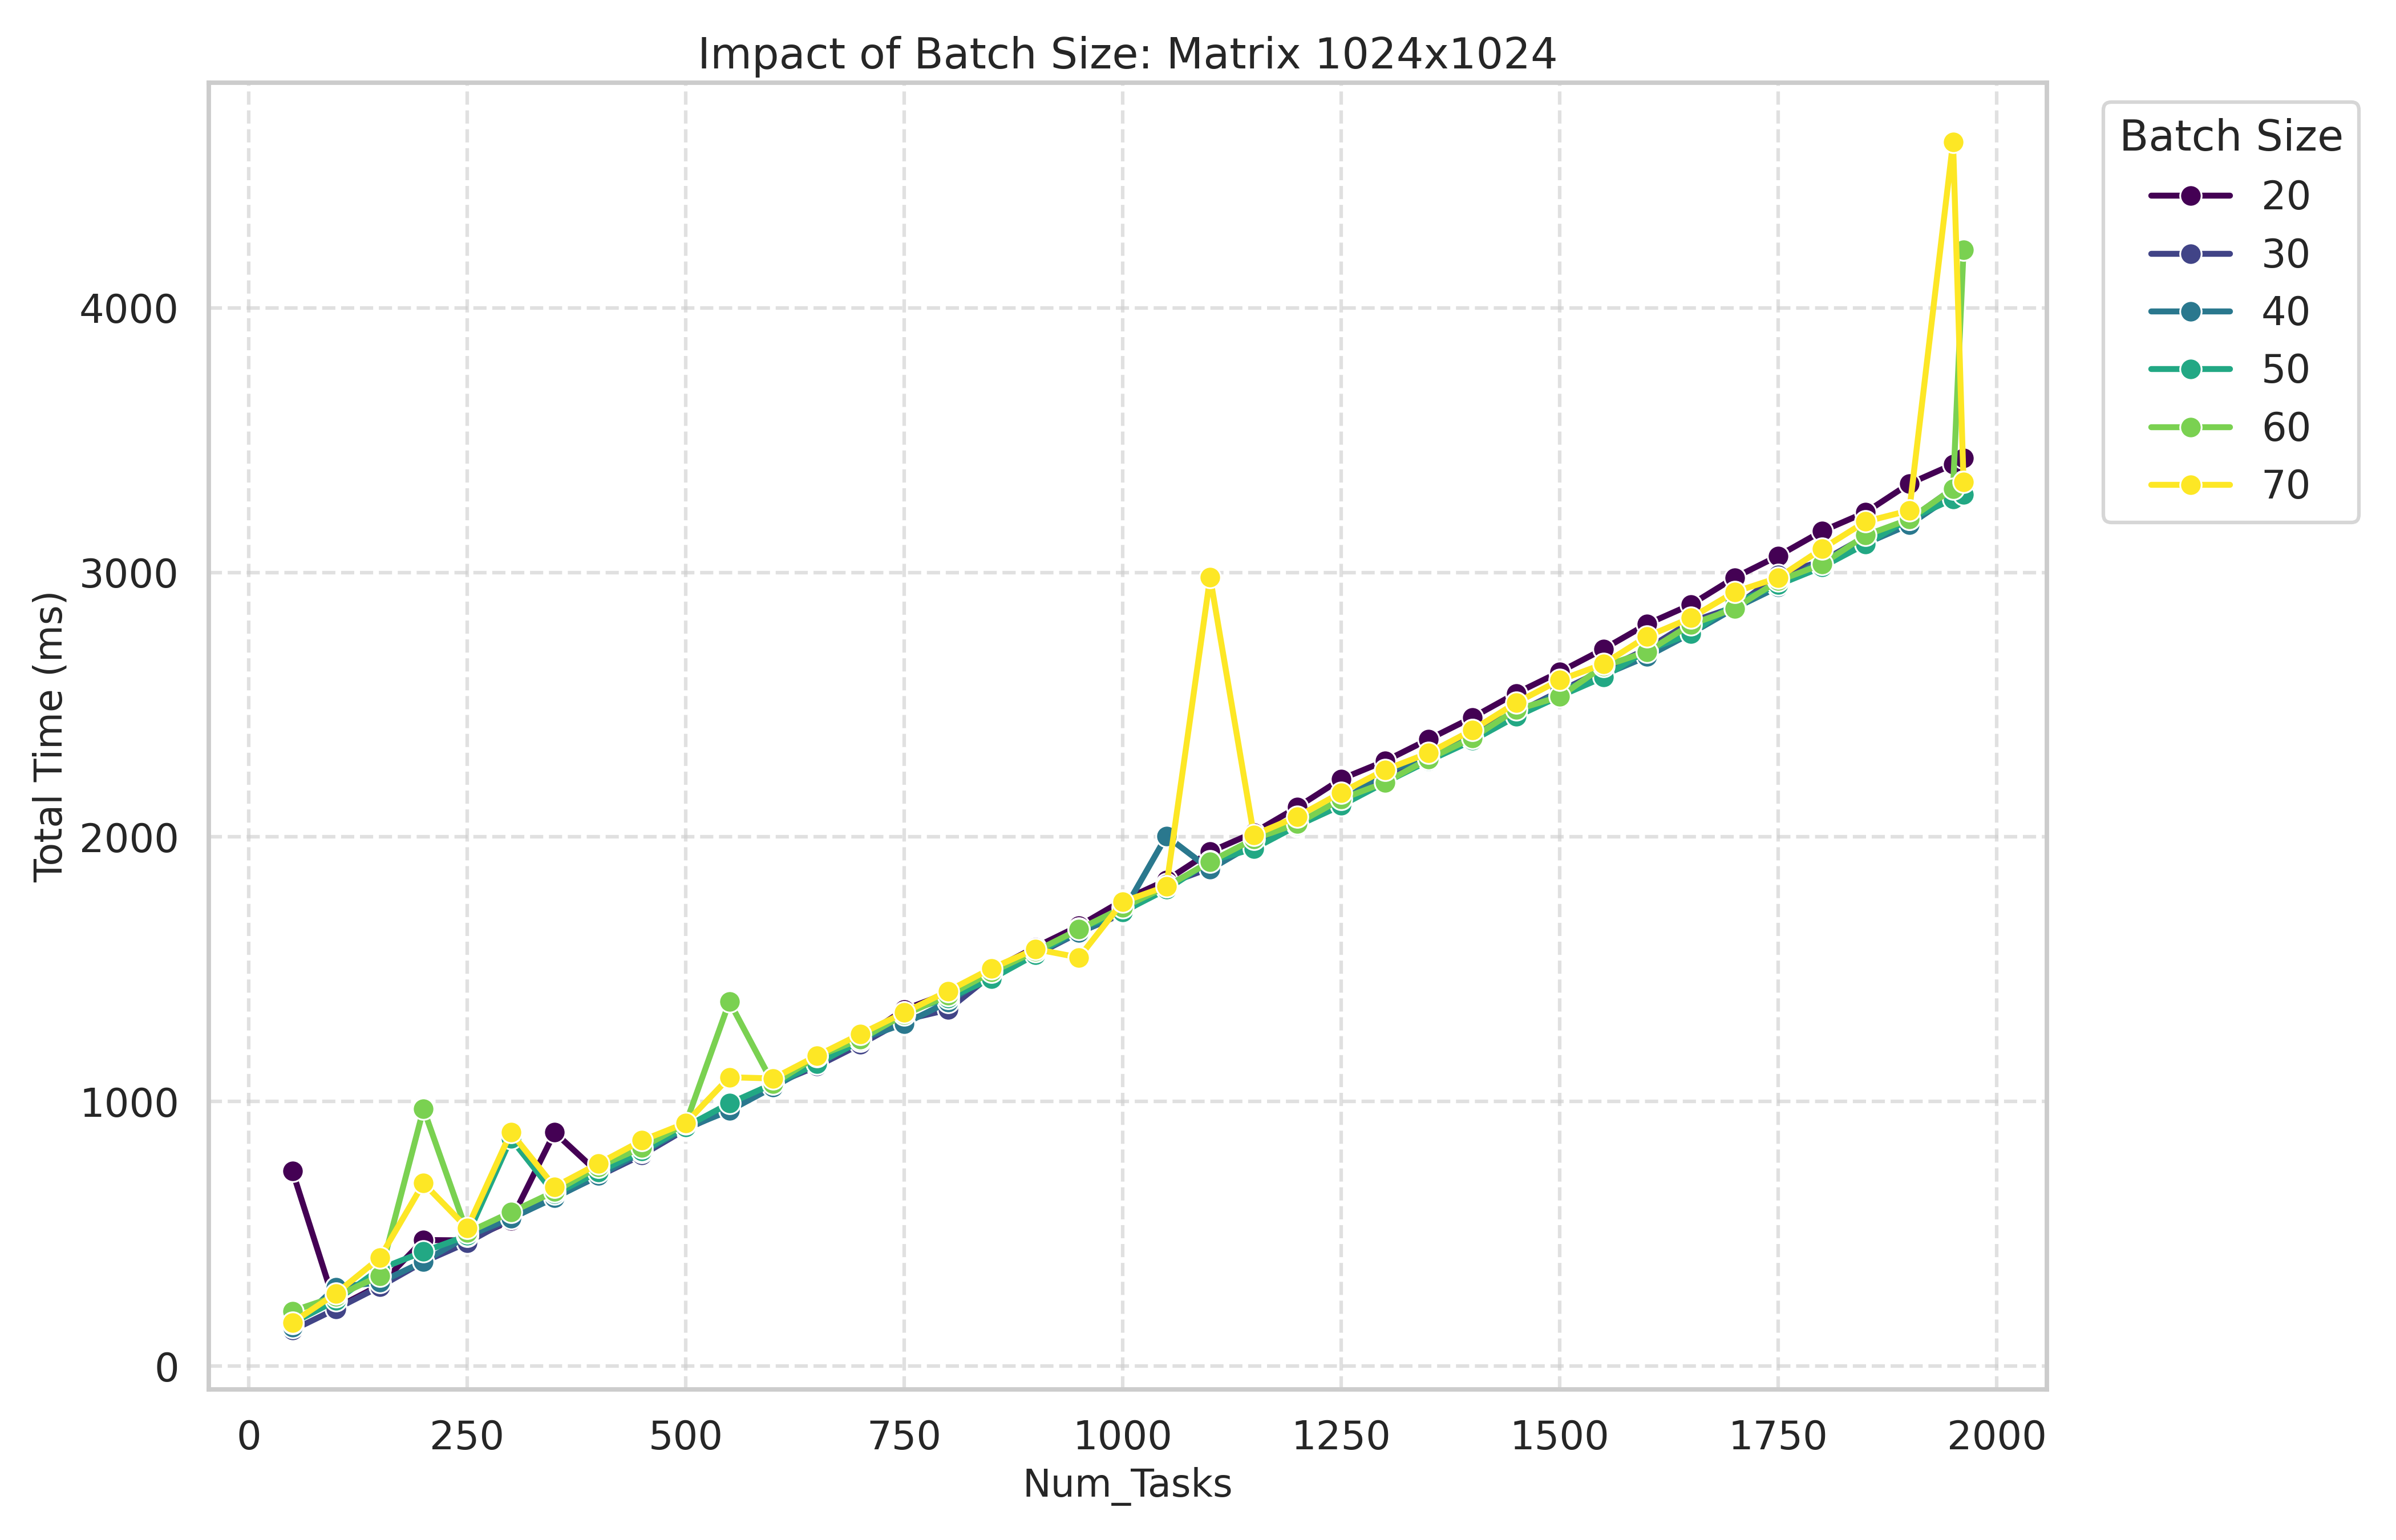
\includegraphics[scale=0.2]{images/results/analysis_batch_S1024.png} 
    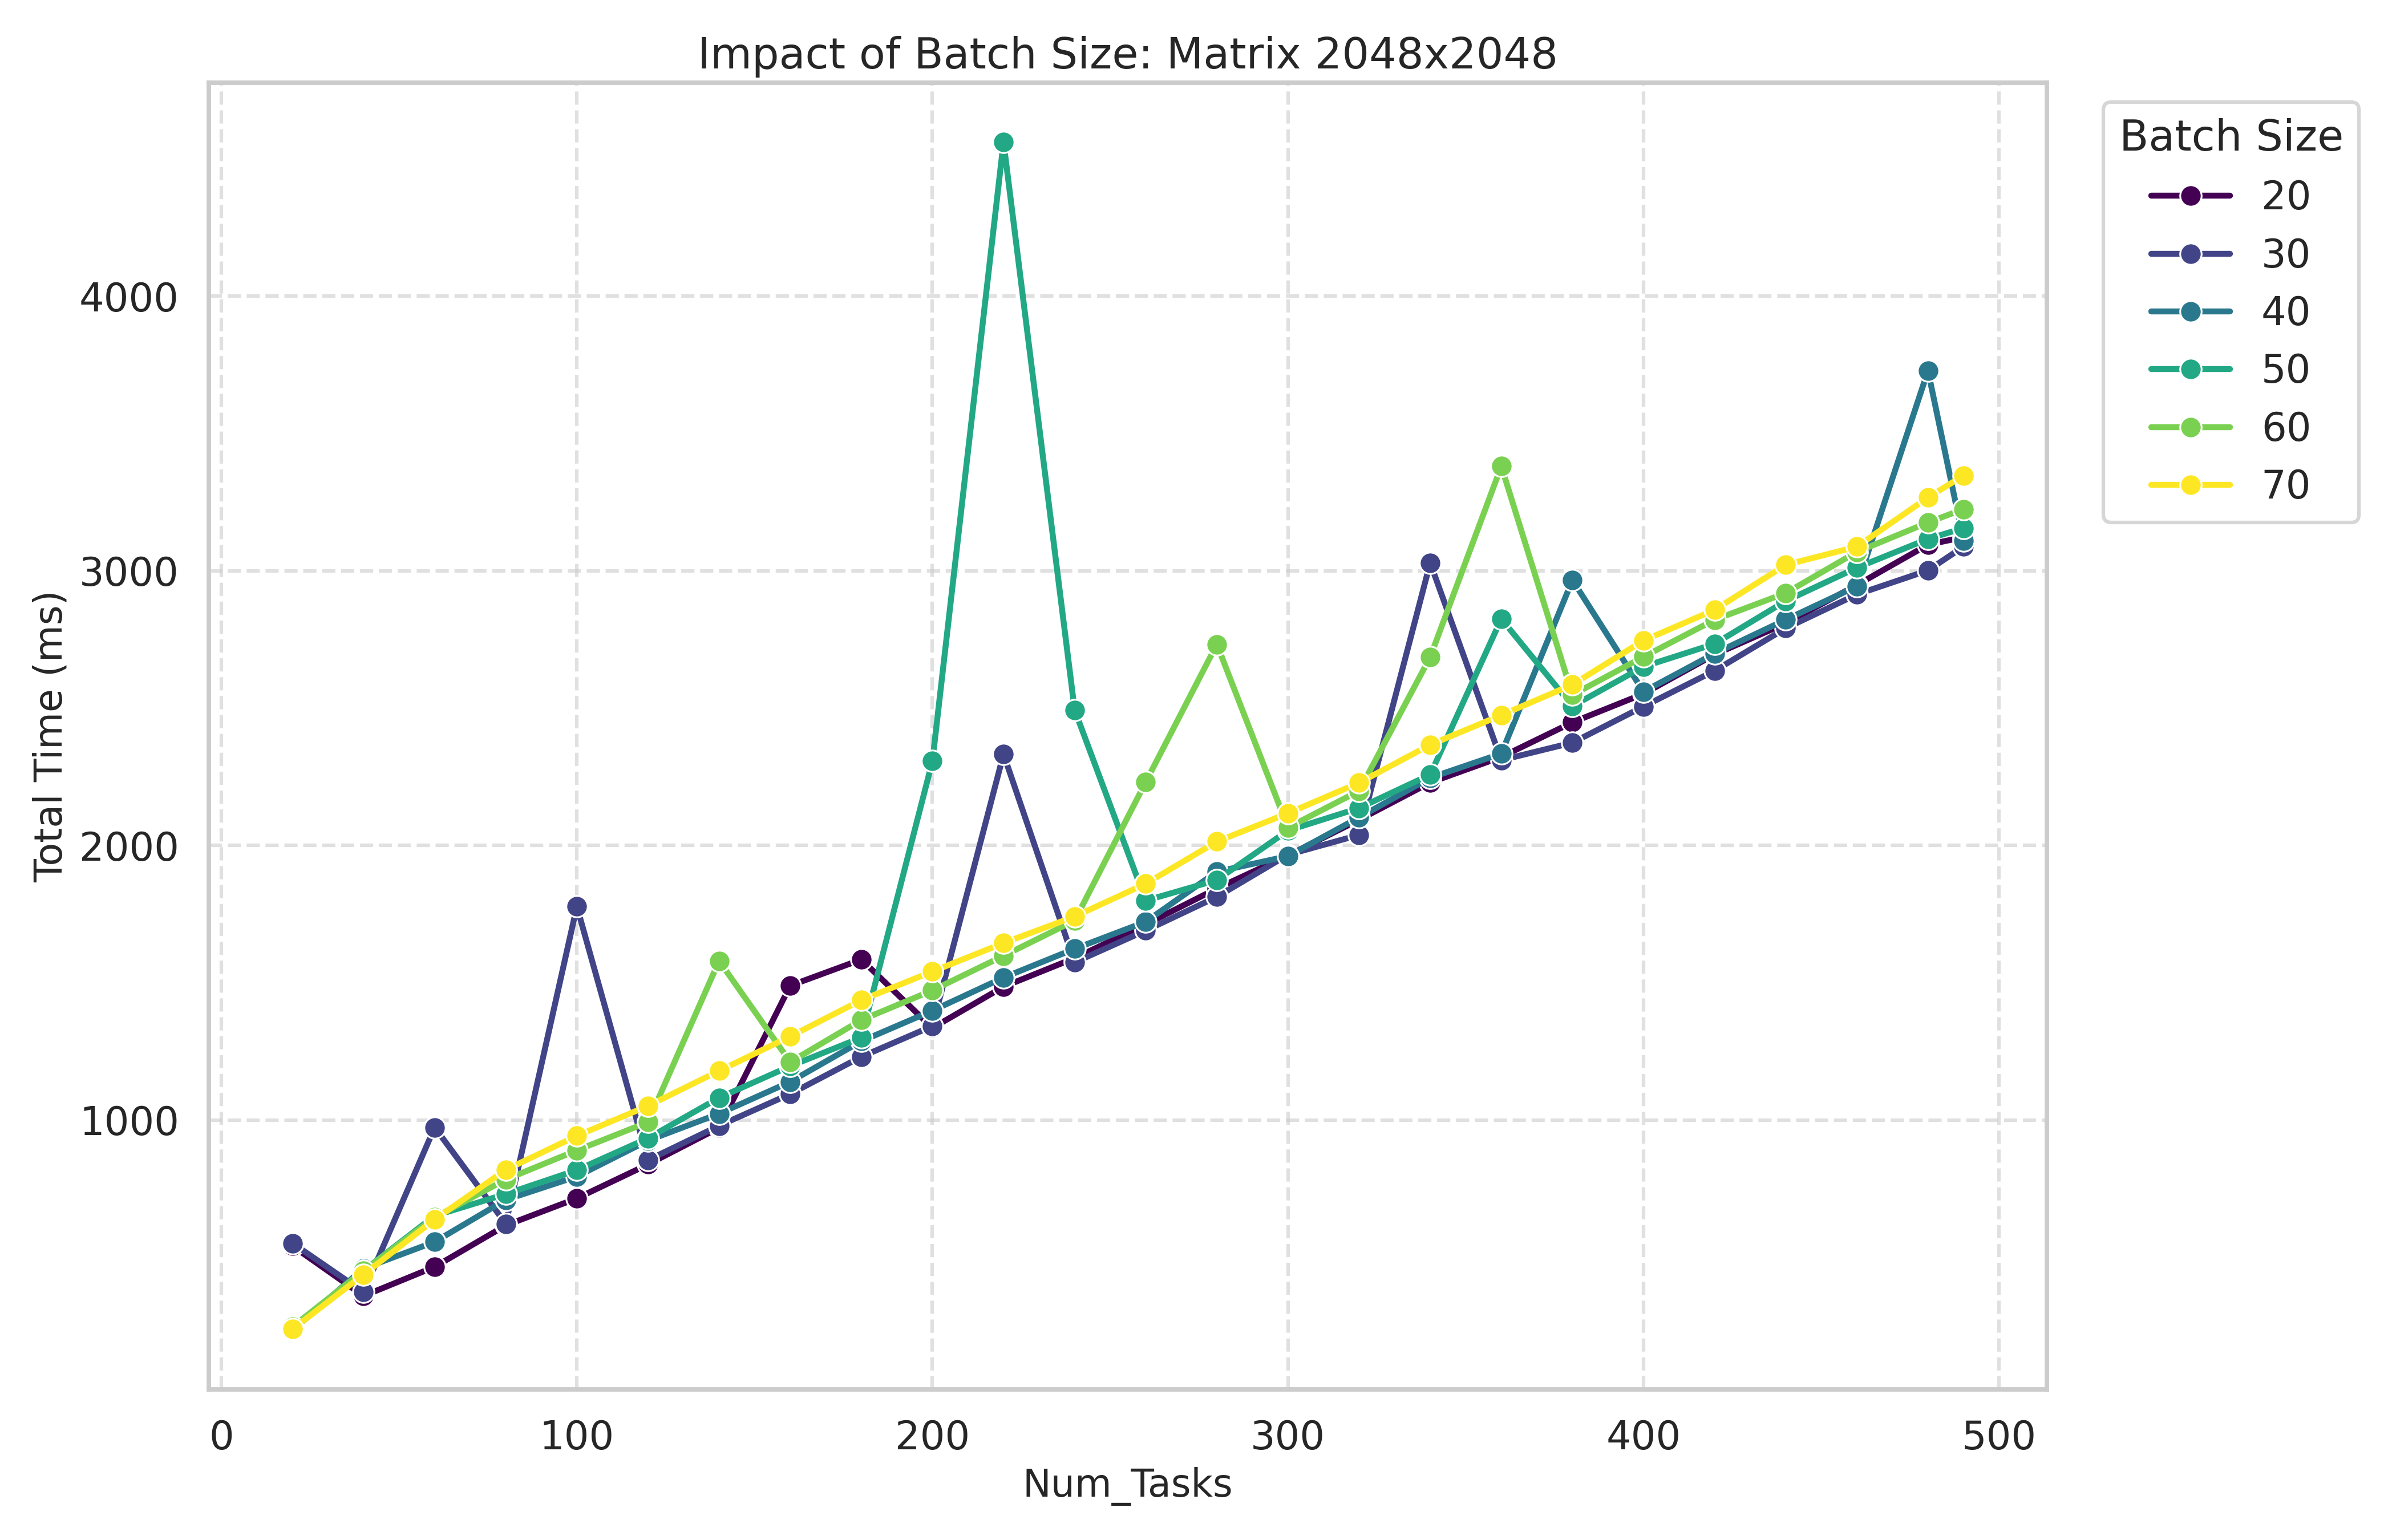
\includegraphics[scale=0.2]{images/results/analysis_batch_S2048.png} 
    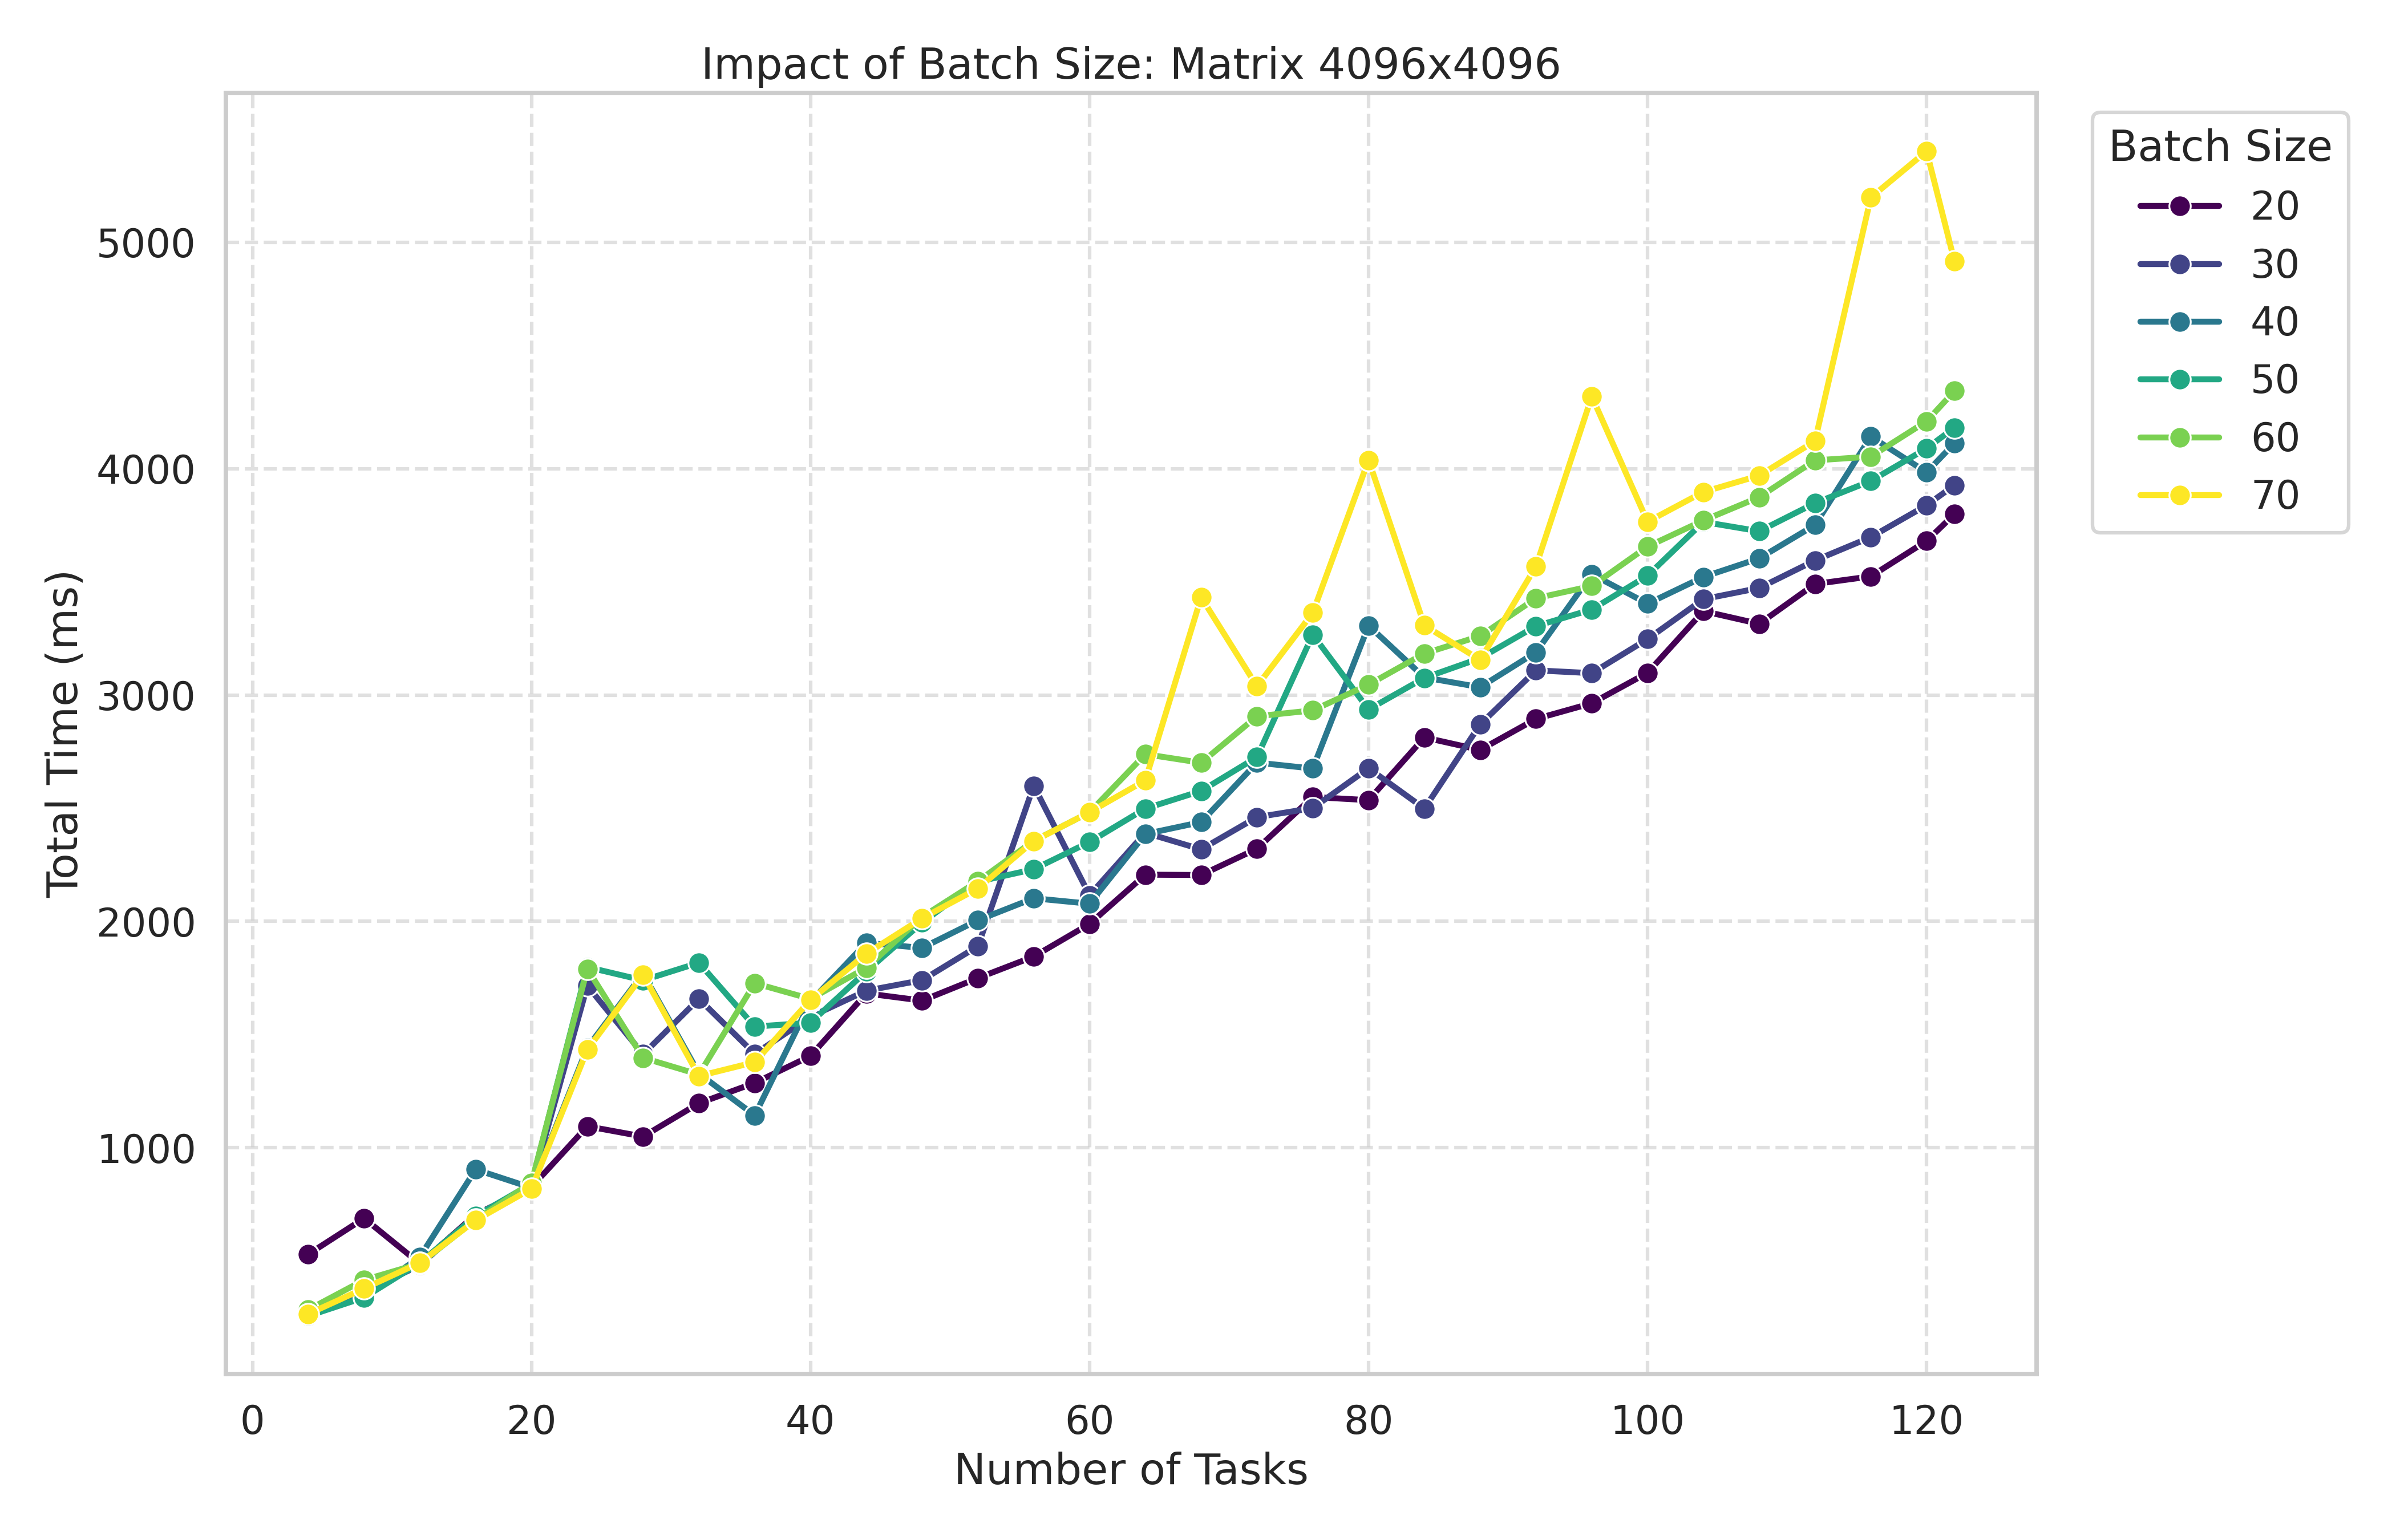
\includegraphics[scale=0.2]{images/results/analysis_batch_S4096.png} 
    \caption{Batch Size Analysis}
    \label{result1}
\end{figure}

As is evident from the graphs in Fig \ref{result1}, a relatively small batch size specifically ranging from 20 to 30 proved to be the most suitable for the selected algorithm and the dataset utilized across each workload. Conversely, it is evident that larger batch sizes frequently result in inaccurate predictions, while inevitably introducing additional overhead to the coordinator adding more time beetween the dispatch of the tasks to the workers.

\clearpage 

\section{Heterogeneous Workloads}
\subsection{Static Heterogeneous}
This test involves streams of matrices with random dimensions ( from 512 to 4096). This represents the most realistic scenario for a general-purpose system, where tasks of varying complexity arrive at the scheduler.

The results of the execution are presented in Fig. \ref{timehetero} and Fig. \ref{energyhetero}:

\begin{figure}[h!]
\centering

\includegraphics[scale=0.3]{images/results/compare_time_Hetero.png}
\caption{Time Comparison: Heterogeneous Stream}
\label{timehetero}
\end{figure}

\begin{figure}[h!]
\centering

\includegraphics[scale=0.3]{images/results/compare_energy_Hetero.png}
\caption{Energy Comparison: Heterogeneous Stream}
\label{energyhetero}
\end{figure}

As shown in Fig. \ref{timehetero}, the difference between the strategies is this case is drastic. The static hetero strategy as the red line proves to be extremely robust, consistently outperforming the single CUDA baseline as the green line. It achieves an average speedup of 1.65x (peaking at 1.85x), demonstrating how this logic achieves a consistent speedup increase while orchestrating the diverse accelerators to handle the heterogeneous workload.

In contrast, the dynamic strategy as the blue line fails to maintain consistent execution times this type of workload. With an average speedup of only 0.42x, it is significantly slower than using the discrete GPU alone. This failure is due to its greedy nature: without looking ahead, it treats a 512×512 matrix and a 4096×4096 matrix as identical tasks, and consistently fails to distribute them efficiently to achieve maximum performance.

The energy analysis in Fig. \ref{energyhetero} mirrors the performance gap already observed:
\begin{itemize}
\item \textbf{Static Strategy}: Consumes on average 112 J, achieving a -17\% energy saving compared to the average CUDA baseline (136 J).
\item \textbf{Dynamic Strategy}: Due to the extremely long execution times, the energy consumption skyrockets to an average of 805 J, with a +490\% increase over the baseline.
\end{itemize}

To better understand these results, we analyze the distribution graphs in Fig. \ref{distribhetero} and Fig. \ref{timedistrhetero}:

\begin{figure}[h!]
\centering

\includegraphics[scale=0.3]{images/results/distrib_tasks_Hetero.png}
\caption{Task Distribution: Heterogeneous Stream}
\label{distribhetero}
\end{figure}

\begin{figure}[h!]
\centering
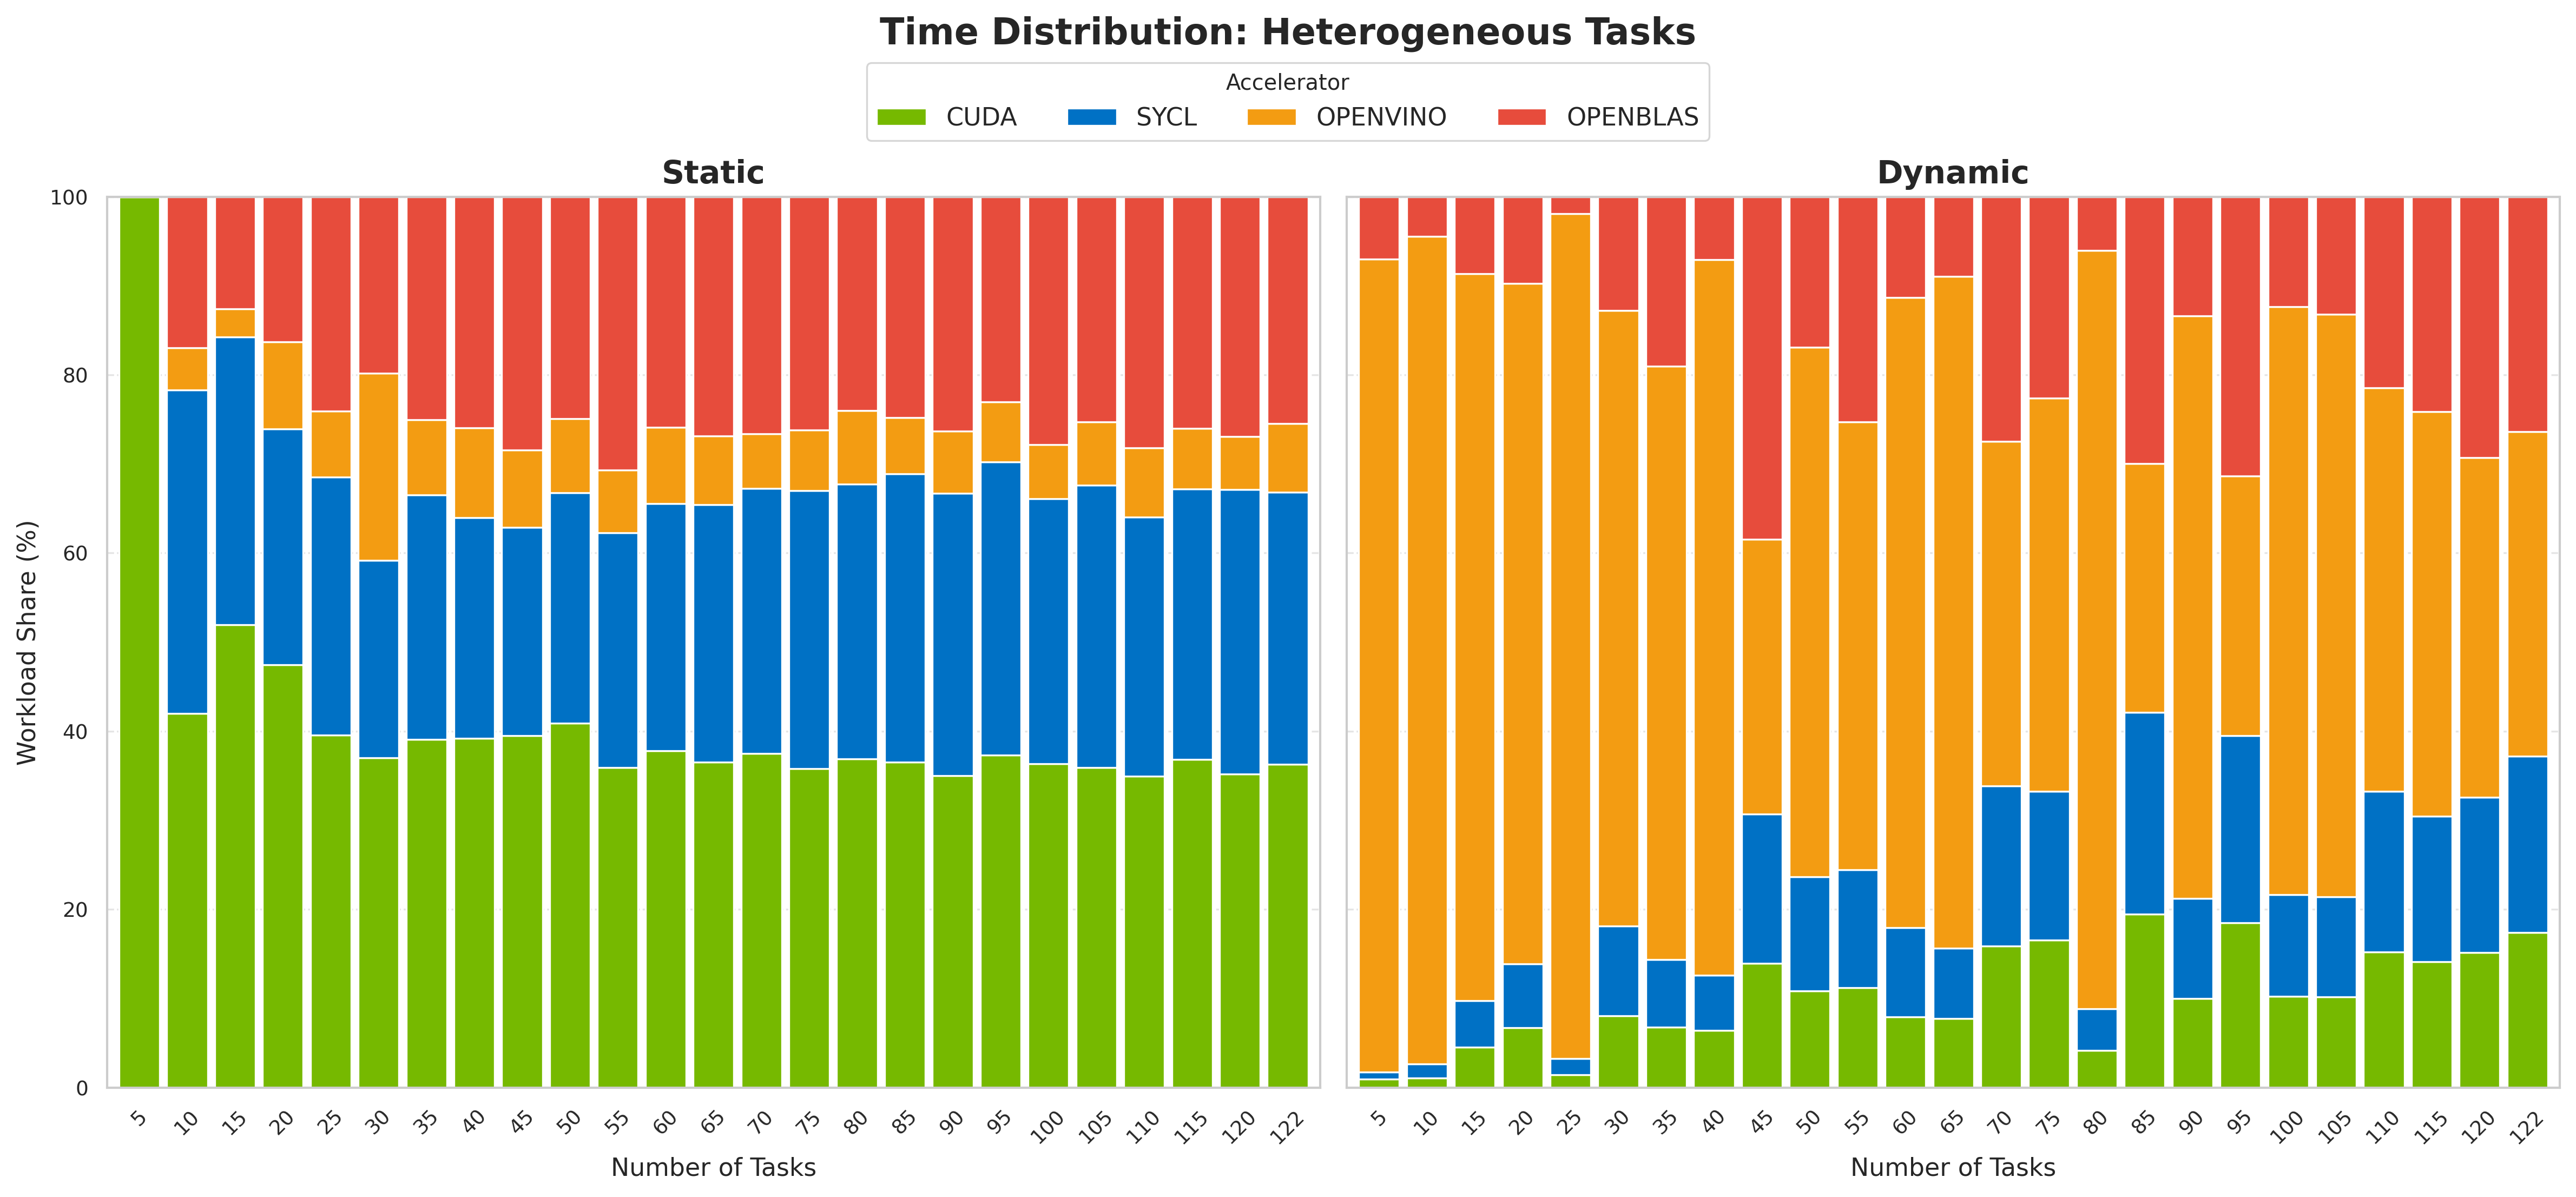
\includegraphics[scale=0.3]{images/results/distrib_Hetero.png}
\caption{Time Distribution: Heterogeneous Stream}
\label{timedistrhetero}
\end{figure}

Regarding the task distribution (see Fig. \ref{distribhetero}), the graph doesn't describe the full scenario since every task has a different weight. However, for the static strategy, we can observe that the number of tasks assigned to each accelerator remains proportional as the total number of tasks increases. This confirms that the strategy is consistent in its decision making logic.

In contrast, the dynamic strategy shows a completely chaotic behavior. Since tasks are assigned to whichever device is free, the distribution varies unpredictably. Unlike the homogeneous tests where the dynamic distribution was relatively stable with smaller tasks, here the randomness of task sizes combined with greedy scheduling leads to a random assignment that changes with every run.

As seen in the Time Distribution (Figure \ref{timedistrhetero}), the CPU and OpenVINO bars are massive. This indicates that the scheduler blindly assigned computationally heavy tasks (e.g., a 4096×4096 matrix) to slow devices simply because they were "free"" at that moment. This creates a massive bottleneck where the powerful GPU finishes its work quickly and sits idle for seconds, waiting for the CPU to finish a single large matrix.

This result conclusively proves that for heterogeneous streams of tasks, smart scheduling with performance prediction is mandatory in this kind of workloads. A simple greedy approach is insufficient and leads to severe performance degradation.

\clearpage 

\subsection{Batch Comparison}
We now present the following graph in Fig. \ref{result_hetero} to illustrate the impact of batch size on the execution times of the static logic under heterogeneous workload conditions:

\begin{figure}[h!]
    \centering
    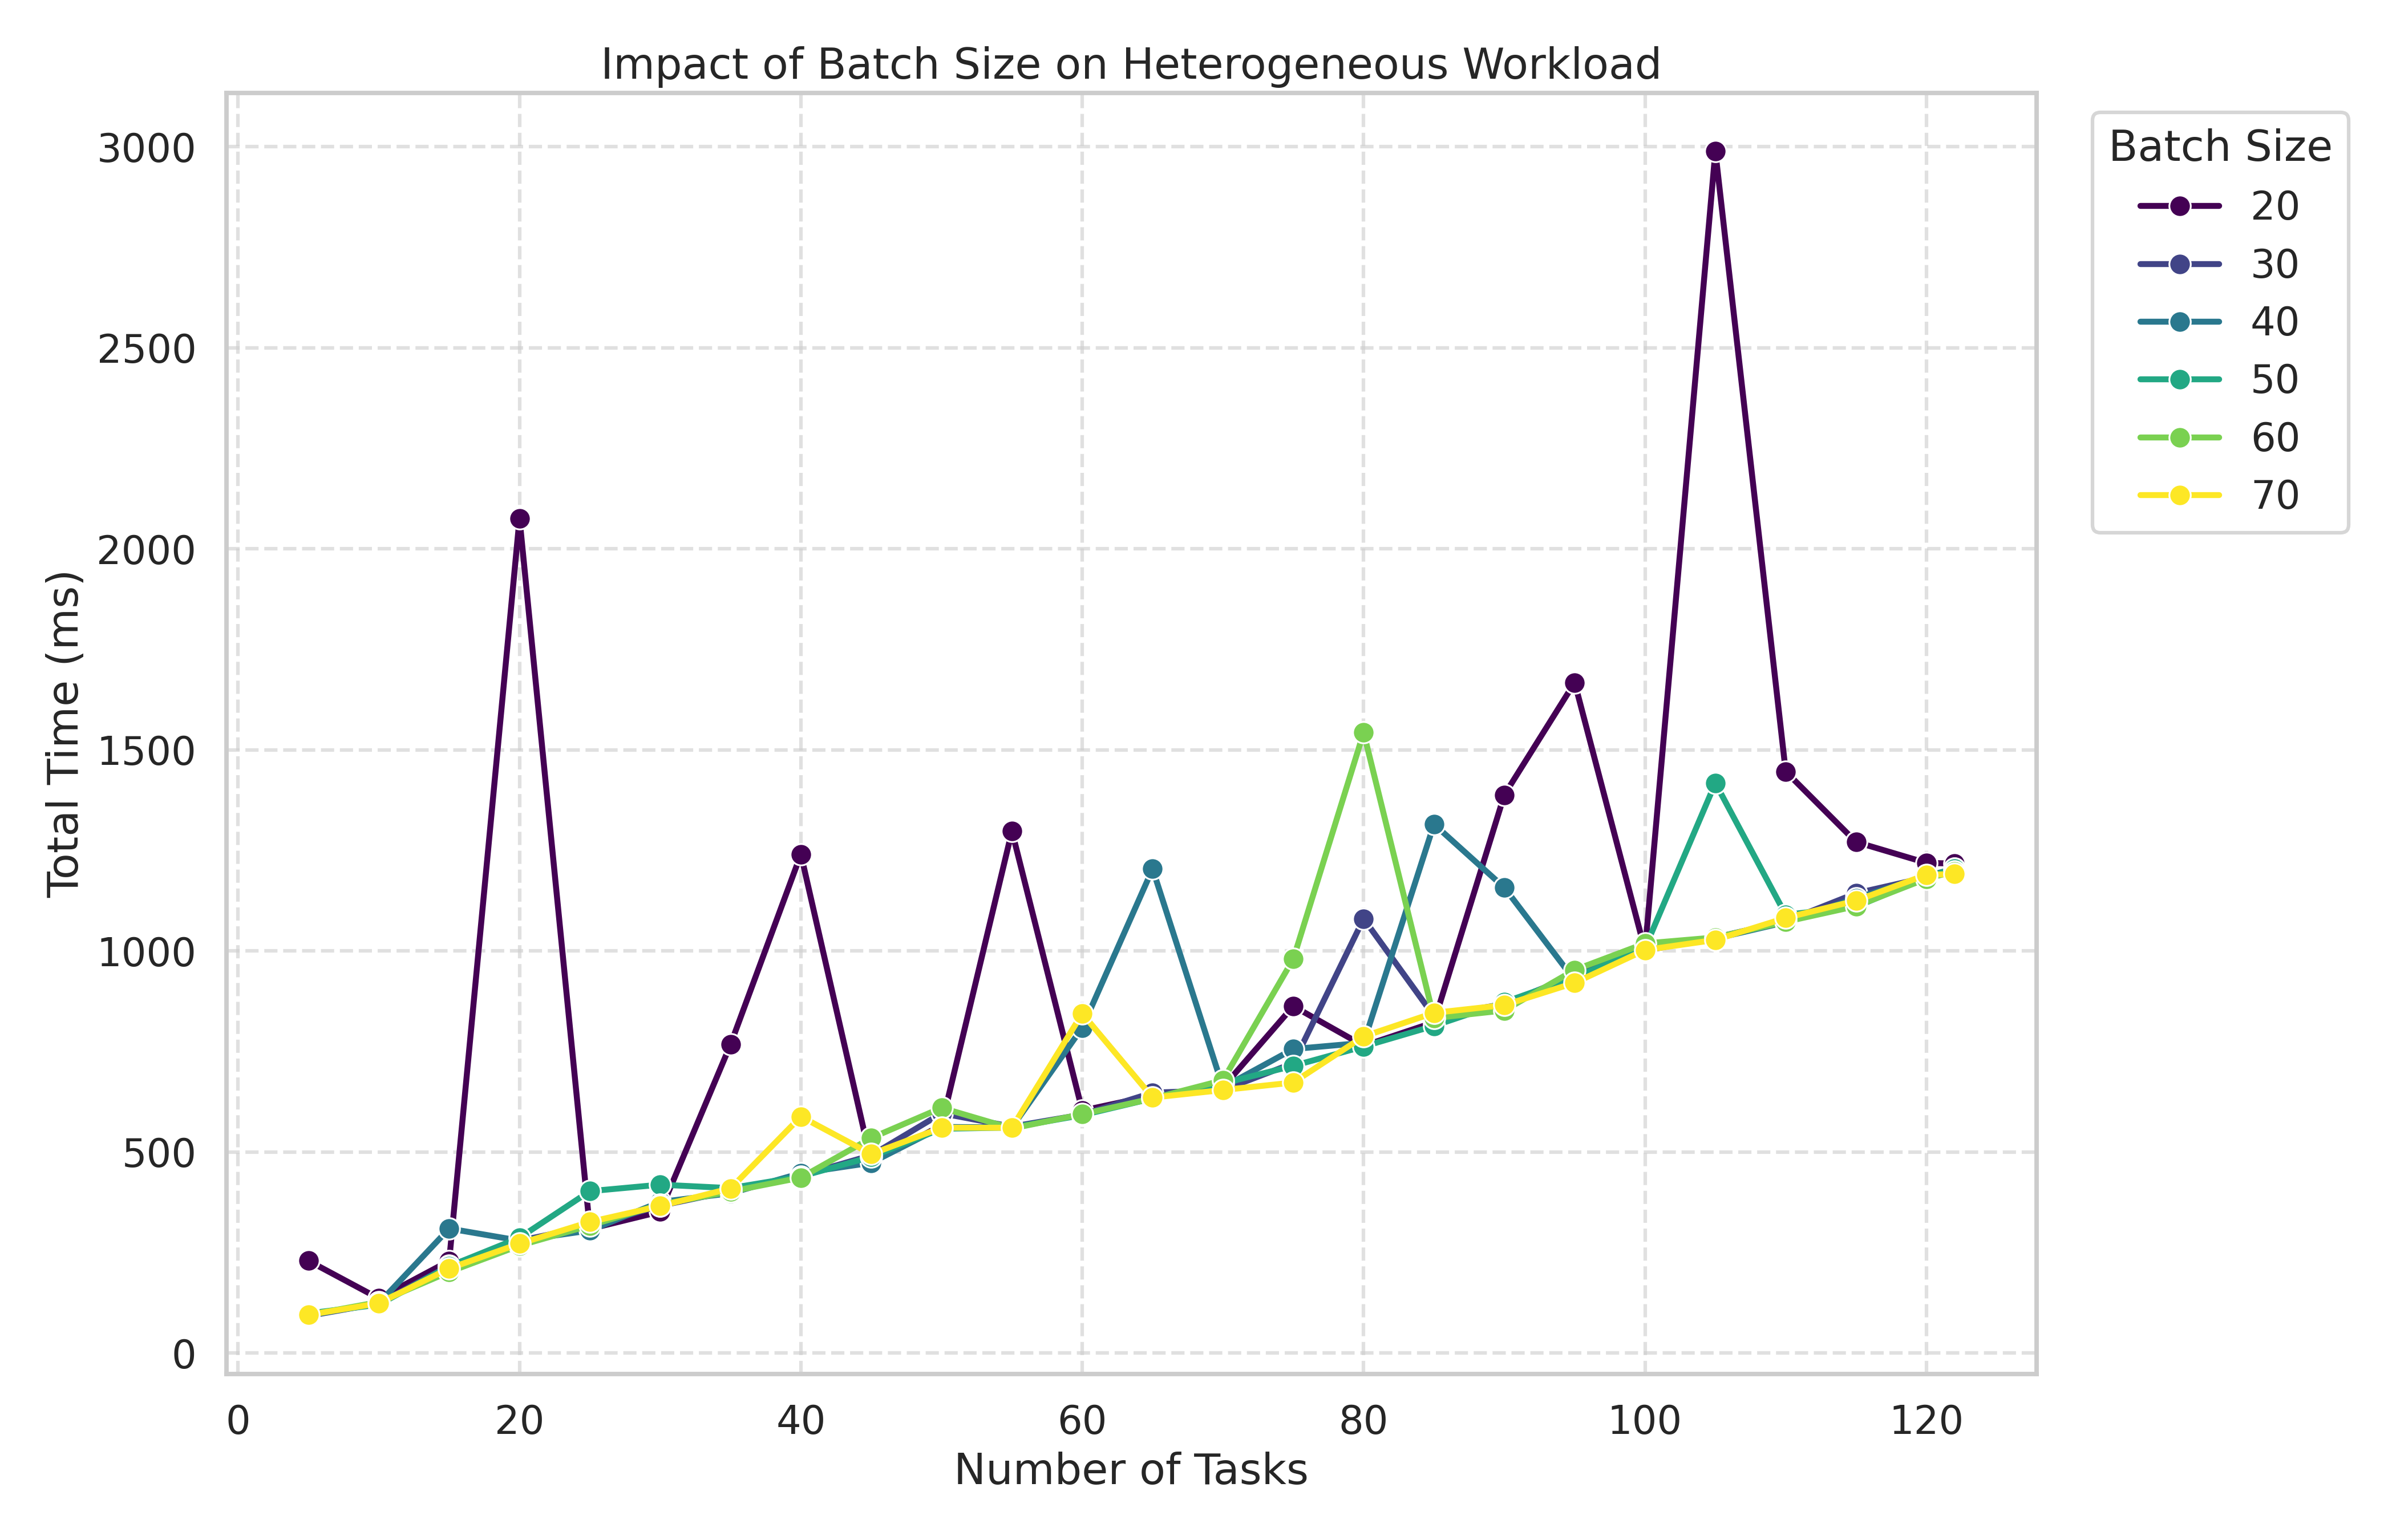
\includegraphics[scale=0.4]{images/results/analysis_batch_hetero.png} 
    \caption{Heterogeneous Batch Size}
    \label{result_hetero}
\end{figure}

As is evident from the graph in Fig \ref{result_hetero}, a relatively large batch size, specifically ranging from 60 to 70, proved to be the most suitable for the static hetero algorithm. Conversely, it is evident that smaller batch sizes (e.g. 20) frequently result in highly unstable execution times, introducing load imbalance due to the high variance of task duration. Larger batches effectively smooth out these variations, allowing the static ratios calculated within the algorithm to converge towards a more efficient distribution of the task, effectively respecting the planned times.

\subsection{Large matrix split}

This scenario involves decomposing a single very large matrix multiplication (where M grows up to 230,000 rows) into smaller sub-tasks (chunks) to fit within device memory limits and distribute the computation.

To provide a fair and meaningful baseline, a simplified version of the splitting logic was implemented. This strategy performs the same chunking operation required to handle the large matrix dimensions but dispatches all chunks exclusively to the NVIDIA GPU (the code can be seen in Appendix \ref{TODO}).

Furthermore, for this specific test case, the OpenVINO backend was excluded. Preliminary tests showed that OpenVINO's performance degrades when handling extremely "rectangular" matrices (very high M, fixed N,K), making it an unsuitable for this specific splitting workload. Our strategy therefore in this test leverages CUDA, SYCL, and OpenBLAS.

The following graphs (Fig. \ref{timelarge}) illustrate the comparison between the Hybrid Split strategy and the CUDA Only baseline:

\begin{figure}[h!]
    \centering
    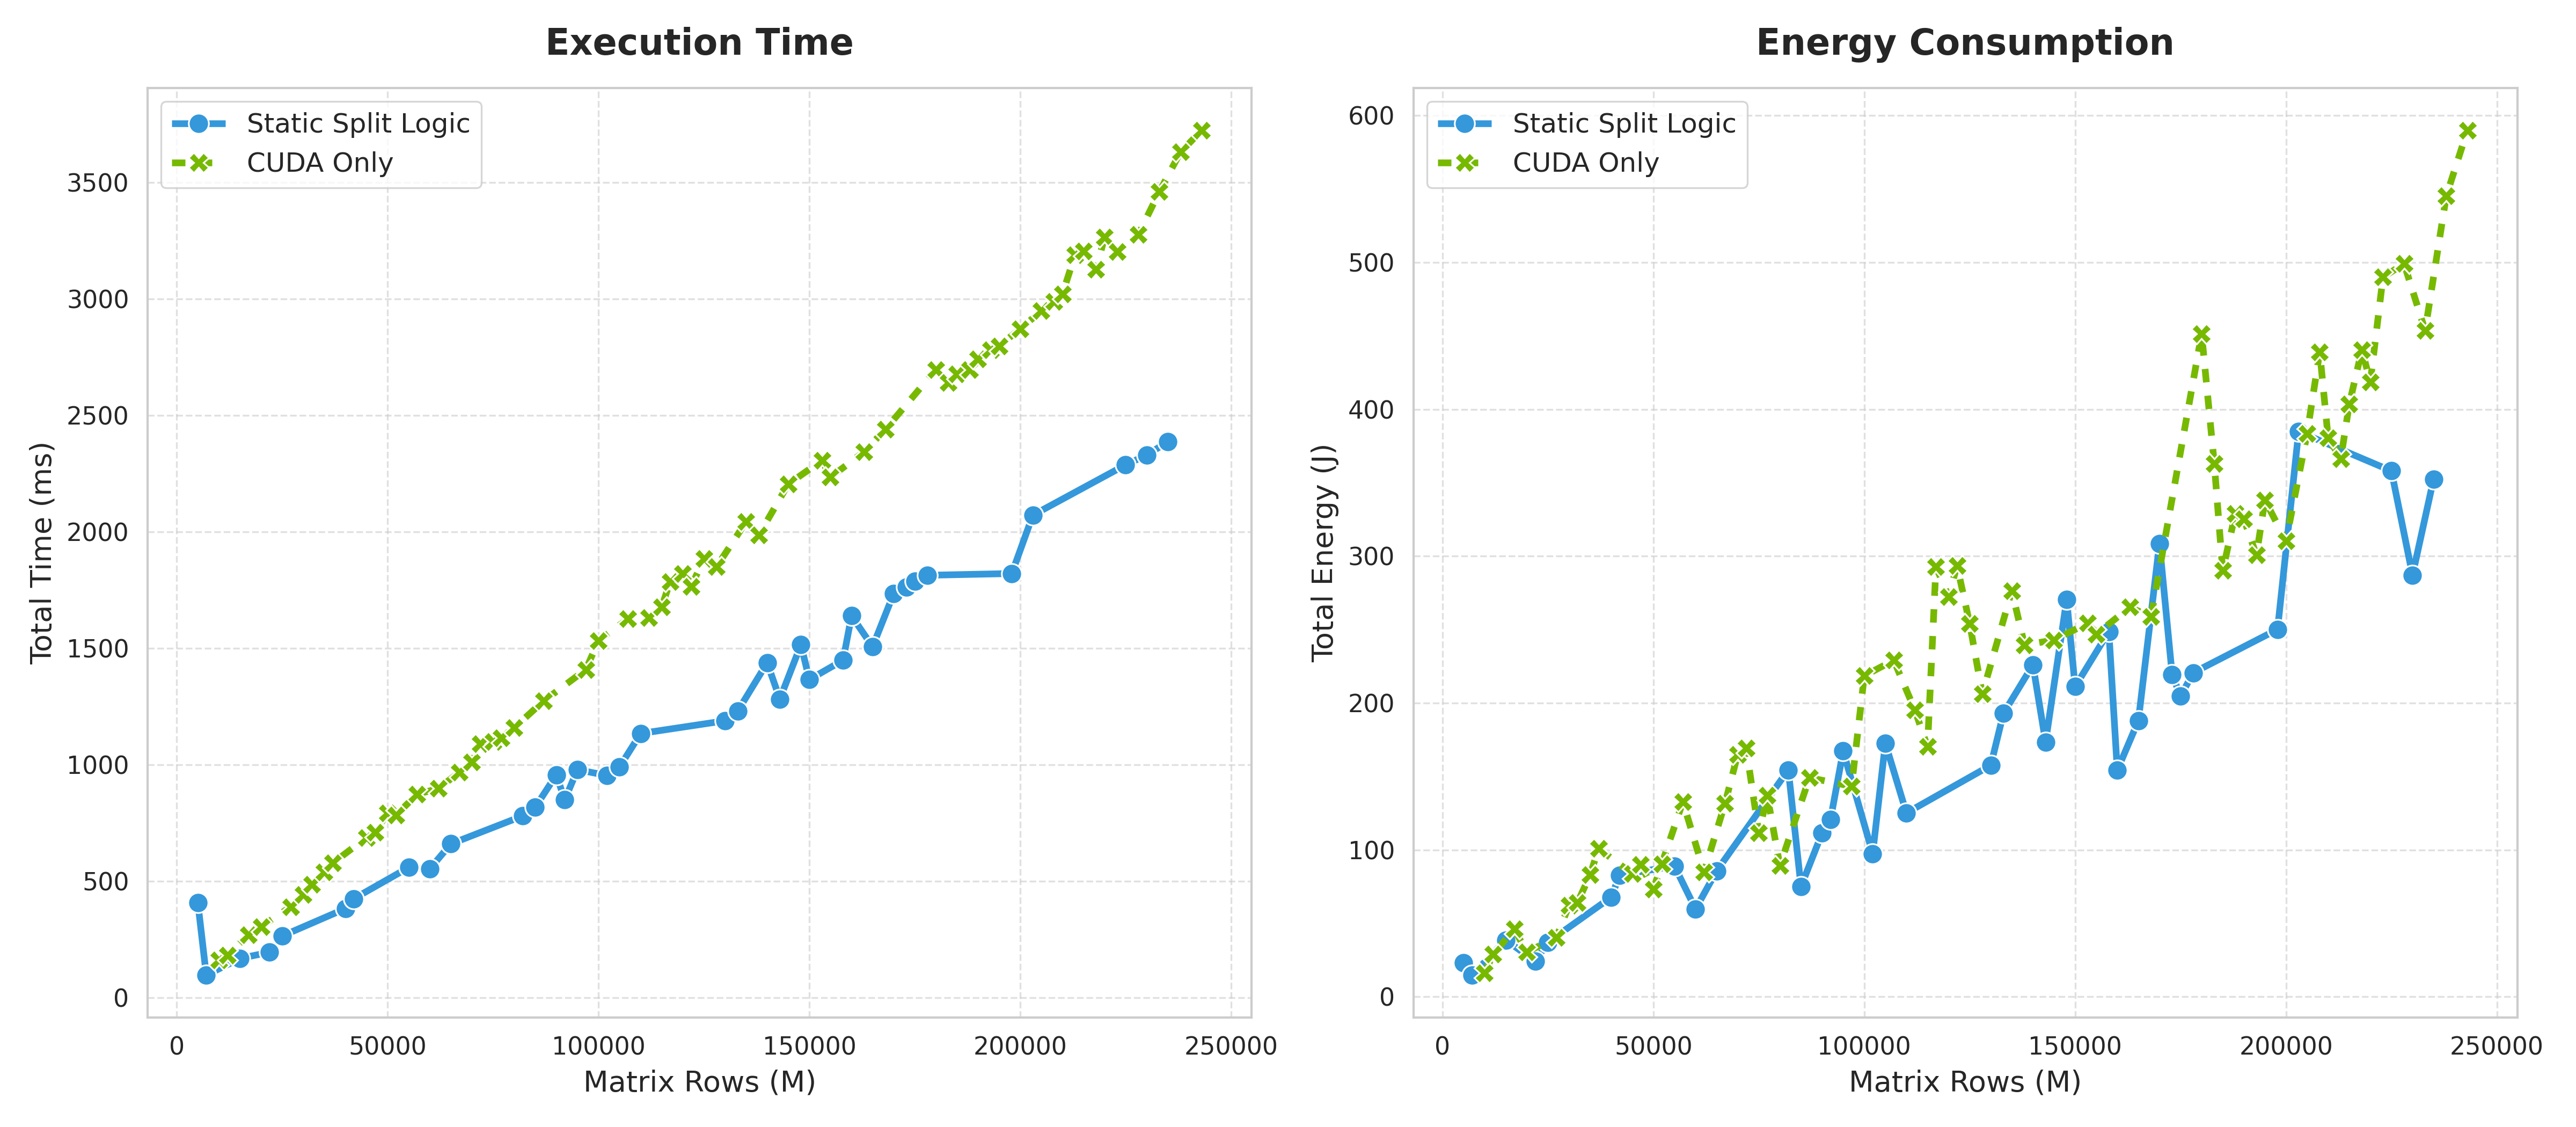
\includegraphics[scale=0.35]{images/results/large_matrix_time_energy.png} 
    \caption{Time and Task Analysis}
    \label{timelarge}
\end{figure}

The execution time comparison on Fig. \ref{timelarge} on the left clearly demonstrates the advantage of the Hybrid split approach. The split logic consistently remains below the green line (CUDA Only), indicating a lower total time to completion across the entire range of matrix sizes. The hybrid strategy achieves an 1.49x average speedup compared to using the GPU alone. In specific configurations the speedup reaches a peak of 2.46x, demonstrating that the combined throughput of the CPU and iGPU can more than double the system's performance for certain problem sizes.

Consumptions wise, the Hybrid strategy also demonstrated superior energy efficiency in some cases (see Fig. \ref{timelarge} on the right): on average, the large static split approach reduced energy consumption by 21\% compared to the CUDA baseline. Furthermore over the entire benchmark, the hybrid strategy consumed 38 J less on average than the 52 J required by the CUDA only execution. This result highlights that finishing the task faster, even by powering up the CPU and iGPU, is often more energy efficient than keeping the discrete GPU active for a longer duration.

\clearpage

\begin{figure}[h!]
    \centering
    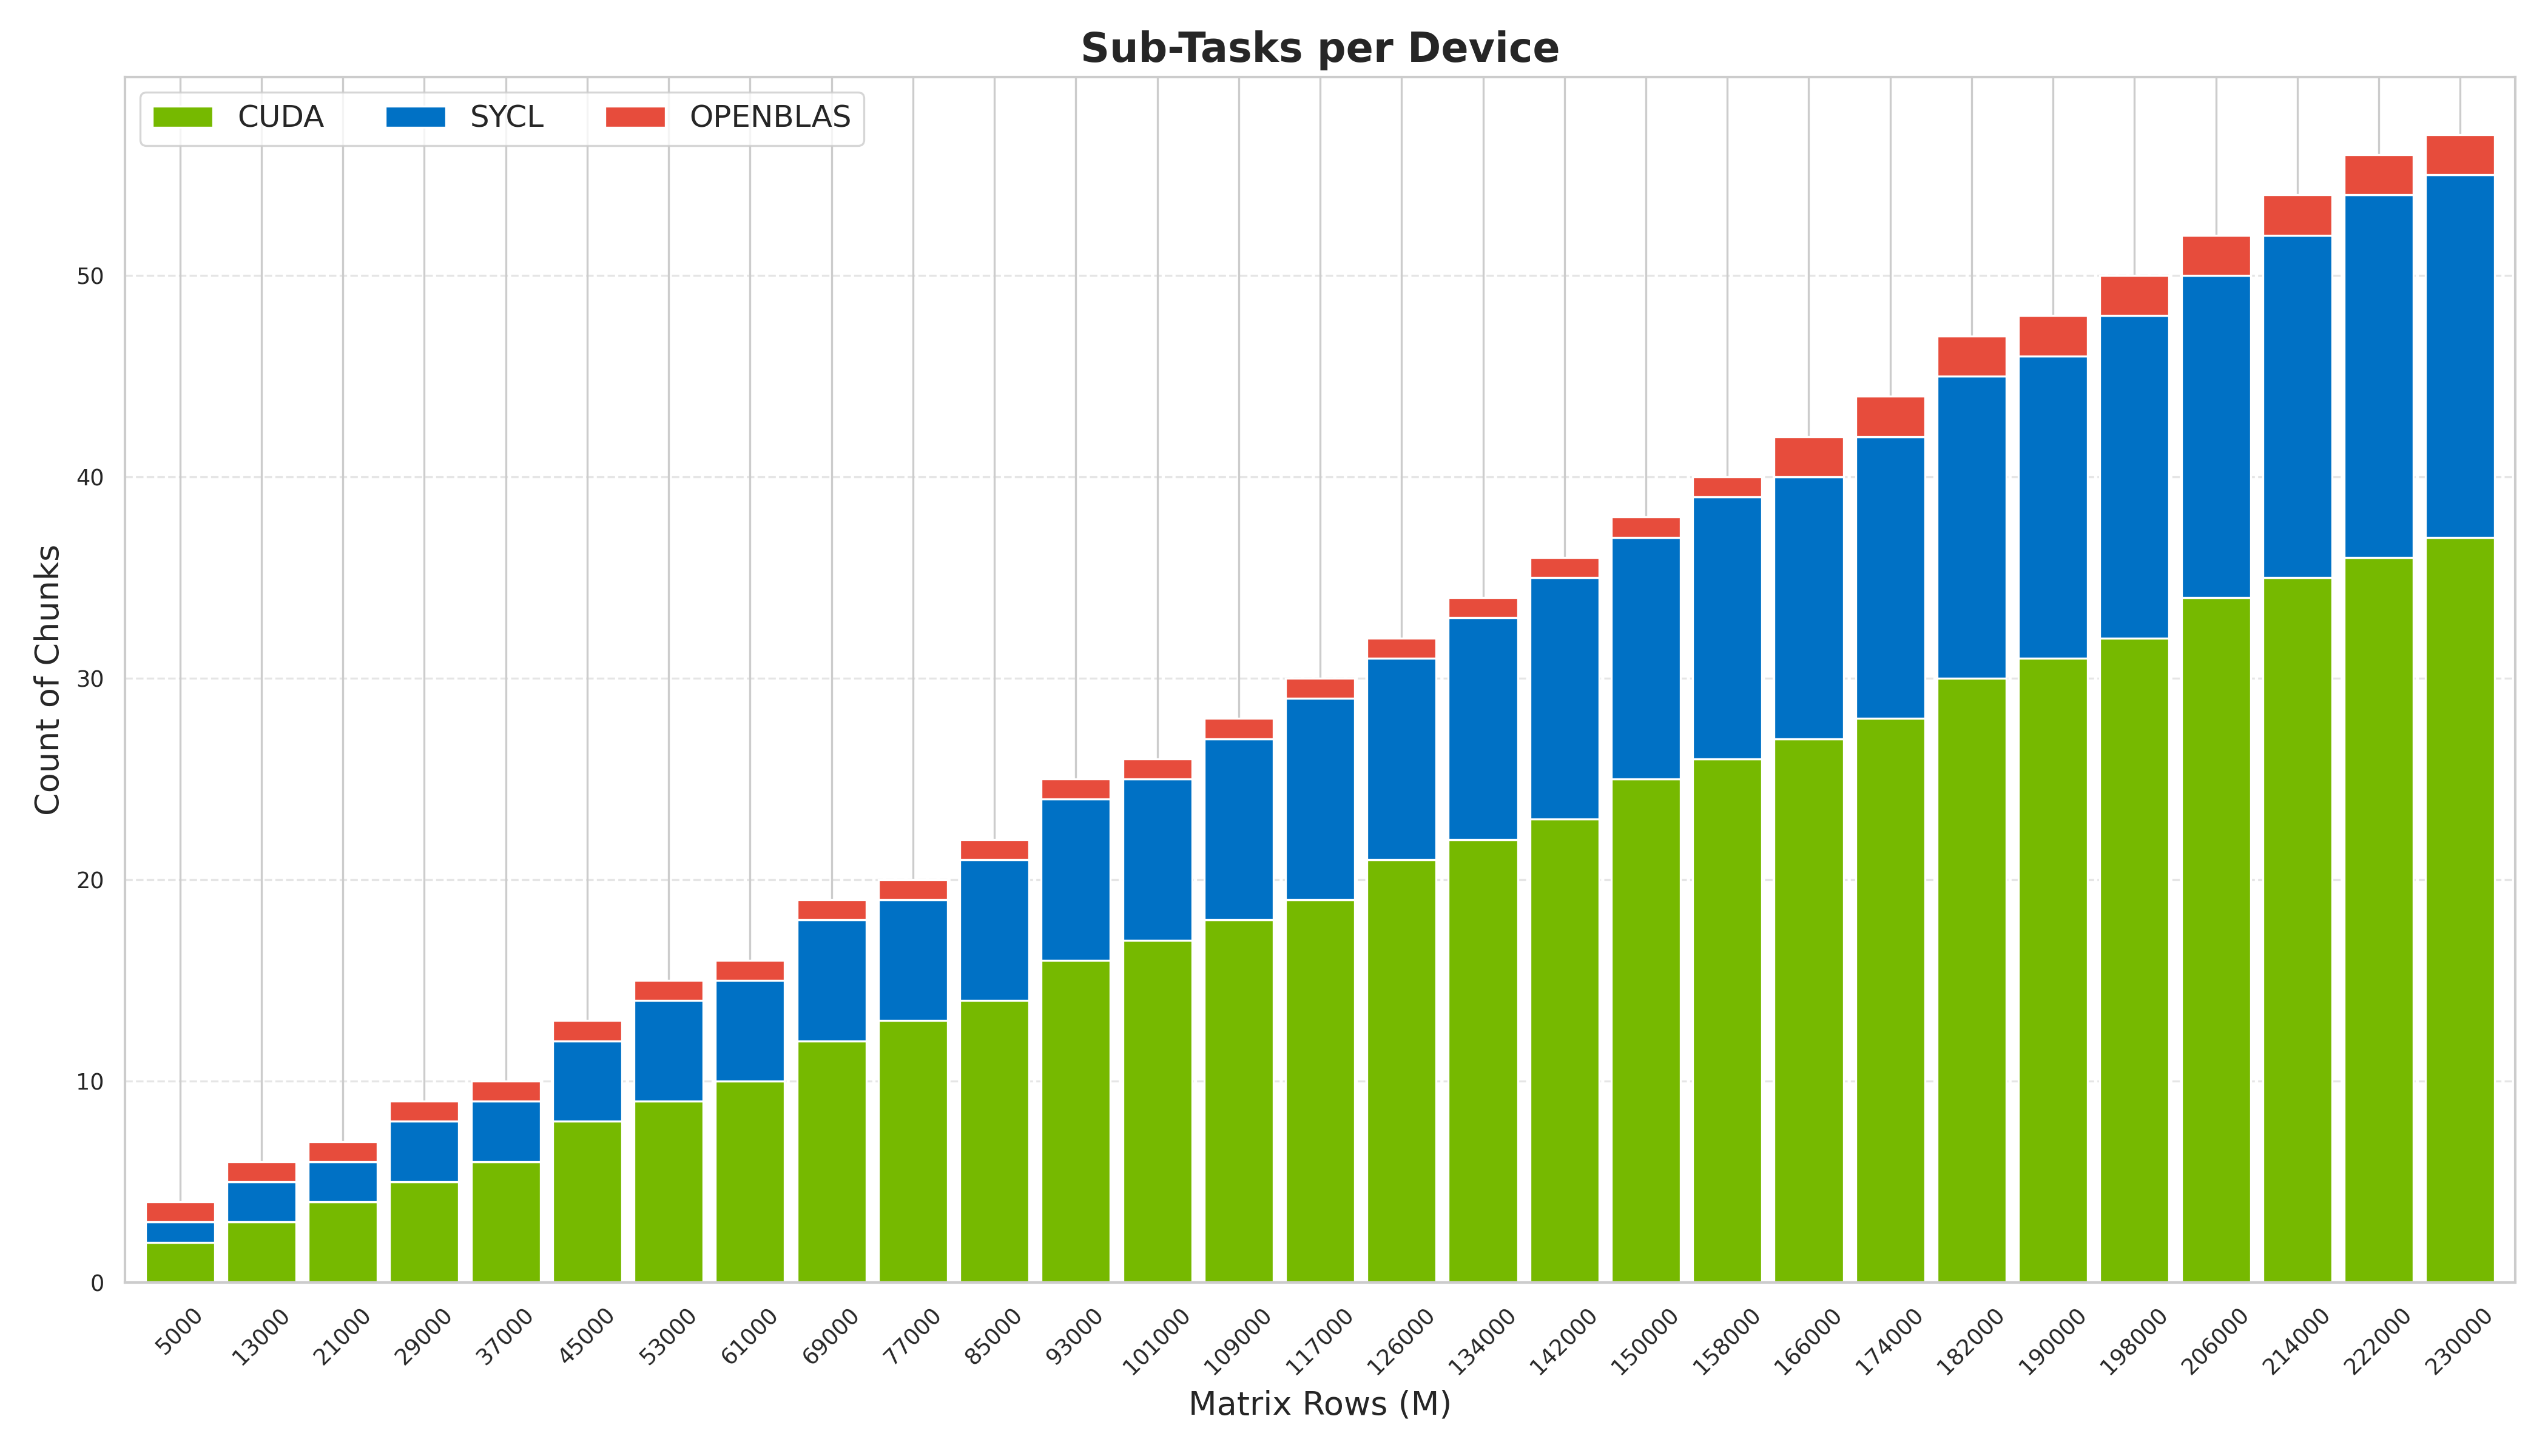
\includegraphics[scale=0.4]{images/results/large_matrix_chunks.png} 
    \caption{Chunk Distribution Analysis}
    \label{chunklarge}
\end{figure}

The load balancing graph on Fig. \ref{chunklarge} provides insight into how the work was distributed. As expected, the powerful CUDA GPU handles the majority of the chunks (approximately 50\% or 60\% of the workload). The remaining of the work is successfully offloaded to the iGPU and CPU backends. This is the direct cause of the observed speedup: by keeping all accelerators active, the system completes the massive calculation faster than the single GPU could.


\appendix

\chapter{Appendix: Source Code}
\label{appendix:source_code}

This appendix contains the source code developed for the AMM Scheduler and the preliminary benchmarks used to analyze the hardware accelerators. The code is organized by project structure.

\section{AMM Scheduler}
The core project of this thesis. It includes the scheduler logic, the task definitions, and the specific backend implementations for CUDA, SYCL, and OpenVINO.

\subsection{Build and Scripts}
\lstinputlisting[language=make, caption={Root (CMakeLists.txt)}]{listings/appendice/amm_scheduler/CMakeLists.txt}
\lstinputlisting[caption={Setup Instructions (setup.txt)}]{listings/appendice/setup.txt}
\lstinputlisting[language=Bash, caption={Build Script (make\_run.sh)}]{listings/appendice/amm_scheduler/make_run.sh}
\lstinputlisting[language=Python, caption={Clangd Utility (merge\_clangd.py)}]{listings/appendice/amm_scheduler/merge_clangd.py}

\subsection{Scheduler}
This section contains the main orchestration logic, including the \texttt{AMScheduler} class, the profiler, and the task definitions.

\lstinputlisting[language=C++, caption={Main (main.cpp)}]{listings/appendice/amm_scheduler/scheduler/main.cpp}
\lstinputlisting[language=C++, caption={Scheduler class (scheduler.hpp)}]{listings/appendice/amm_scheduler/scheduler/scheduler.hpp}
\lstinputlisting[language=C++, caption={Task definitions (tasks.hpp)}]{listings/appendice/amm_scheduler/scheduler/tasks.hpp}
\lstinputlisting[language=C++, caption={profiler.hpp}]{listings/appendice/amm_scheduler/scheduler/profiler.hpp}
\lstinputlisting[language=C++, caption={performancemap.hpp}]{listings/appendice/amm_scheduler/scheduler/performancemap.hpp}
\lstinputlisting[language=C++, caption={OpenBlass Implementation (cpu.hpp)}]{listings/appendice/amm_scheduler/scheduler/cpu.hpp}
\lstinputlisting[language=C++, caption={sharedbuffer.hpp}]{listings/appendice/amm_scheduler/scheduler/sharedbuffer.hpp}
\lstinputlisting[language=C++, caption={config.hpp}]{listings/appendice/amm_scheduler/scheduler/config.hpp}
\lstinputlisting[language=C++, caption={tests.hpp}]{listings/appendice/amm_scheduler/scheduler/tests.hpp}

\subsection{Backend: CUDA}
Implementation of the NVIDIA GPU backend.
\lstinputlisting[language=C++, caption={CUDA Runner (runner.cu)}]{listings/appendice/amm_scheduler/cuda/runner.cu}
\lstinputlisting[language=C++, caption={CUDA Wrapper (cuda\_wrapper.h)}]{listings/appendice/amm_scheduler/cuda/cuda_wrapper.h}

\subsection{Backend: SYCL}
Implementation of the Intel Integrated Graphics backend via SYCL (OneAPI).
\lstinputlisting[language=C++, caption={SYCL Runner (runner.cpp)}]{listings/appendice/amm_scheduler/sycl/runner.cpp}
\lstinputlisting[language=C++, caption={SYCL Wrapper (sycl\_wrapper.h)}]{listings/appendice/amm_scheduler/sycl/sycl_wrapper.h}

\subsection{Backend: OpenVINO}
Implementation of the Intel NPU backend via OpenVINO.
\lstinputlisting[language=C++, caption={OpenVINO Runner (runner.cpp)}]{listings/appendice/amm_scheduler/openvino/runner.cpp}
\lstinputlisting[language=C++, caption={OpenVINO Wrapper (ov\_wrapper.h)}]{listings/appendice/amm_scheduler/openvino/ov_wrapper.h}

\subsubsection{OpenCV test}
\lstinputlisting[language=C++, caption={OpenCV Video Test (opencv\_test.hpp)}]{listings/appendice/amm_scheduler/scheduler/opencv_test.hpp}

\clearpage
\section{Benchmarks}
This section includes the standalone benchmarks developed to study the behavior of the accelerators before the integration into the main scheduler.

\subsection{CUDA Benchmark}
\lstinputlisting[language=C++, caption={CUDA Main (main.cu)}]{listings/appendice/gpu_benchmark/src/main.cu}

\lstinputlisting[language=C++, caption={GEMM Runner (gem\_runner.cu)}]{listings/appendice/gpu_benchmark/src/benchmarks/gem_runner.cu}
\lstinputlisting[language=C++, caption={Memory Runner (mem\_runner.cu)}]{listings/appendice/gpu_benchmark/src/benchmarks/mem_runner.cu}

%\lstinputlisting[language=C++, caption={Power Header (power.hpp)}]{listings/appendice/gpu_benchmark/src/include/benchmark/power.hpp}
%\lstinputlisting[language=C++, caption={Helper Functions (help\_func.hpp)}]{listings/appendice/gpu_benchmark/src/include/benchmark/help_func.hpp}

\subsection{OpenVINO Benchmark}
\lstinputlisting[language=C++, caption={Openvino Main (main.cpp)}]{listings/appendice/npu_benchmark/main.cpp}
\lstinputlisting[language=make, caption={Openvino Makefile}]{listings/appendice/npu_benchmark/Makefile}

\subsection{SYCL Benchmark}
\lstinputlisting[language=C++, caption={SYCL Main (main.cpp)}]{listings/appendice/sycl_benchmark/main.cpp}
\lstinputlisting[language=C++, caption={SYCL Makefile)}]{listings/appendice/sycl_benchmark/Makefile}



\bibliographystyle{plain}
\bibliography{chapters/Bibliografia.bib}

\end{document}
% -----------------------------------------------------------------
